

\chapter{Studies pertaining to the monitoring of isoflurane and sevoflurane by proton transfer reaction mass spectrometry}\label{chapter:iso}
\markboth{Anaesthetics in PTR-MS}{}


This chapter contains PTR-MS results from isoflurane and sevoflurane acquired for reproducibility purposes that contributed to the discussion and publication of the following paper:

\fullcite{ISOF_paper}


The experimental data published in this paper is that acquired by the first author, including PTR-MS investigations of desflurane and enflurane.
%
Here only PTR-MS results of the reaction 
of isoflurane with (H$_2$O)$_n$H$_3$O$^+$ and O$_2^+$ 
and of sevoflurane with (H$_2$O)$_n$H$_3$O$^+$ 
are provided, including the reagent ion signal intensities related to each experiment.
%
These are shown in figures \ref{fig:isof_h3o} - \ref{fig:sevo_h3o_h}.
%
%Note that the small differences (i.e. <3\%) in the relationship between the drift tube voltage and the \textit{E/N} are due to the hollow cathode and the reactor being set at slightly different pressures to optimise the reagent ion signal in each case. 
%
%
%The drift voltage range is different to those shown in other chapters because for the measurements presented in this chapter another PTR-MS instrument was used.
%
The structure of isoflurane and sevoflurane are shown in \autoref{fig:iso}.



\section{PTR-MS results of isoflurane and sevoflurane}


\begin{figure}
\sidesubfloat[]{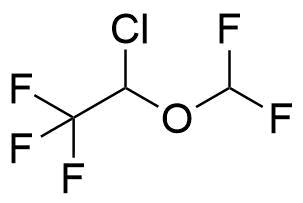
\includegraphics[width=0.15\textwidth]{pics/ISOF_structure.png}}
\sidesubfloat[]{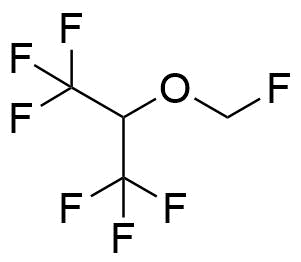
\includegraphics[width=0.15\textwidth]{pics/SEVO_struct.png}}
  \caption{Structure of (a) isoflurane and (b) sevoflurane.}
  \label{fig:iso}
\end{figure}




%\subsection{PTR-MS}
%\subsubsection{Isoflurane: proton transfer mode}


\begin{figure}%[h]
\centering
\sidesubfloat[]{
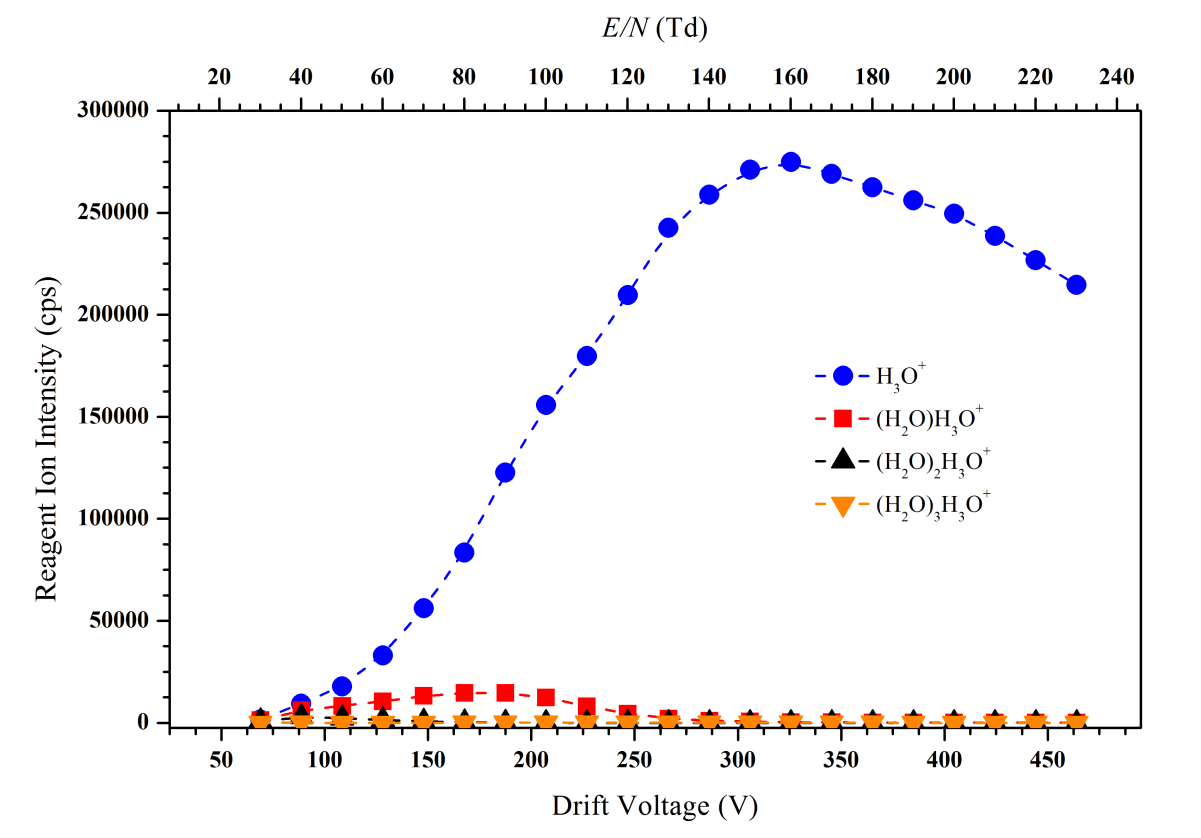
\includegraphics[width=0.60\linewidth]{pics/ISOF/ANAESTH_001.png}
}

\sidesubfloat[]{
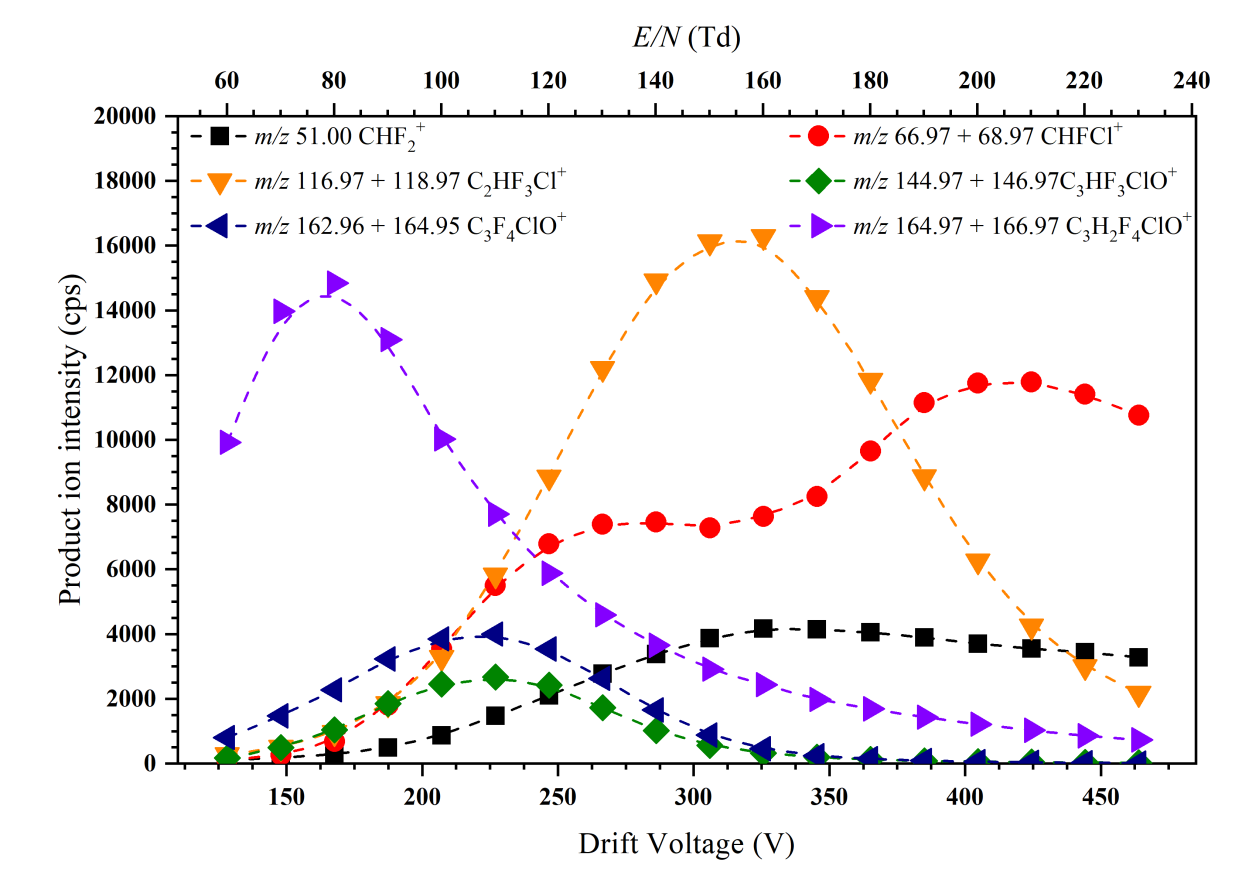
\includegraphics[width=0.60\linewidth]{pics/ISOF/ANAESTH_003.png}
}

\sidesubfloat[]{
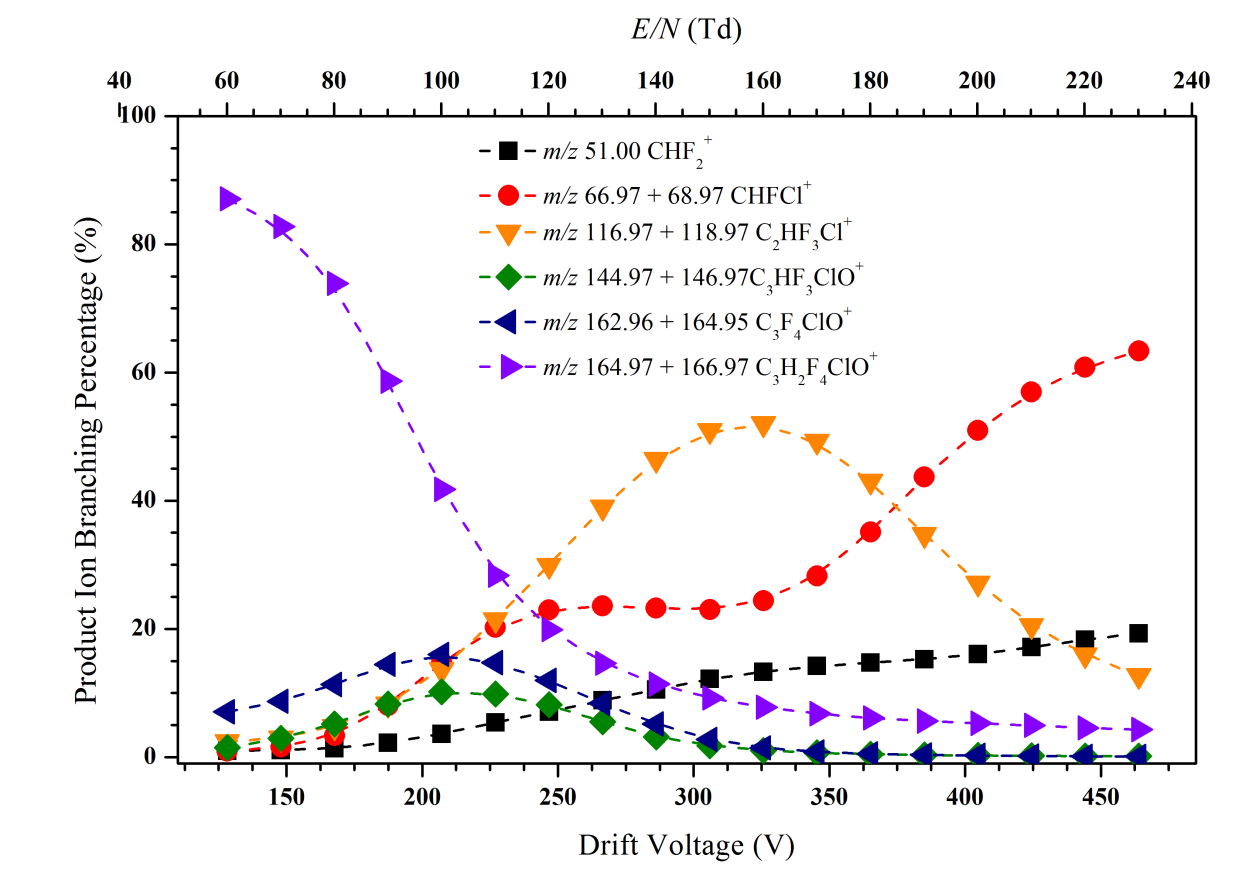
\includegraphics[width=0.60\linewidth]{pics/ISOF/ANAESTH_002.png}
}

\caption{(a) Reagent ions intensity plot and product ions  (b) intensity and (c) distribution plots from the reaction of isoflurane and (H$_2$O)$_n$H$_3$O$^+$ in dry conditions.}
\label{fig:isof_h3o}
\end{figure}

\begin{figure}%[h]
\centering
\sidesubfloat[]{
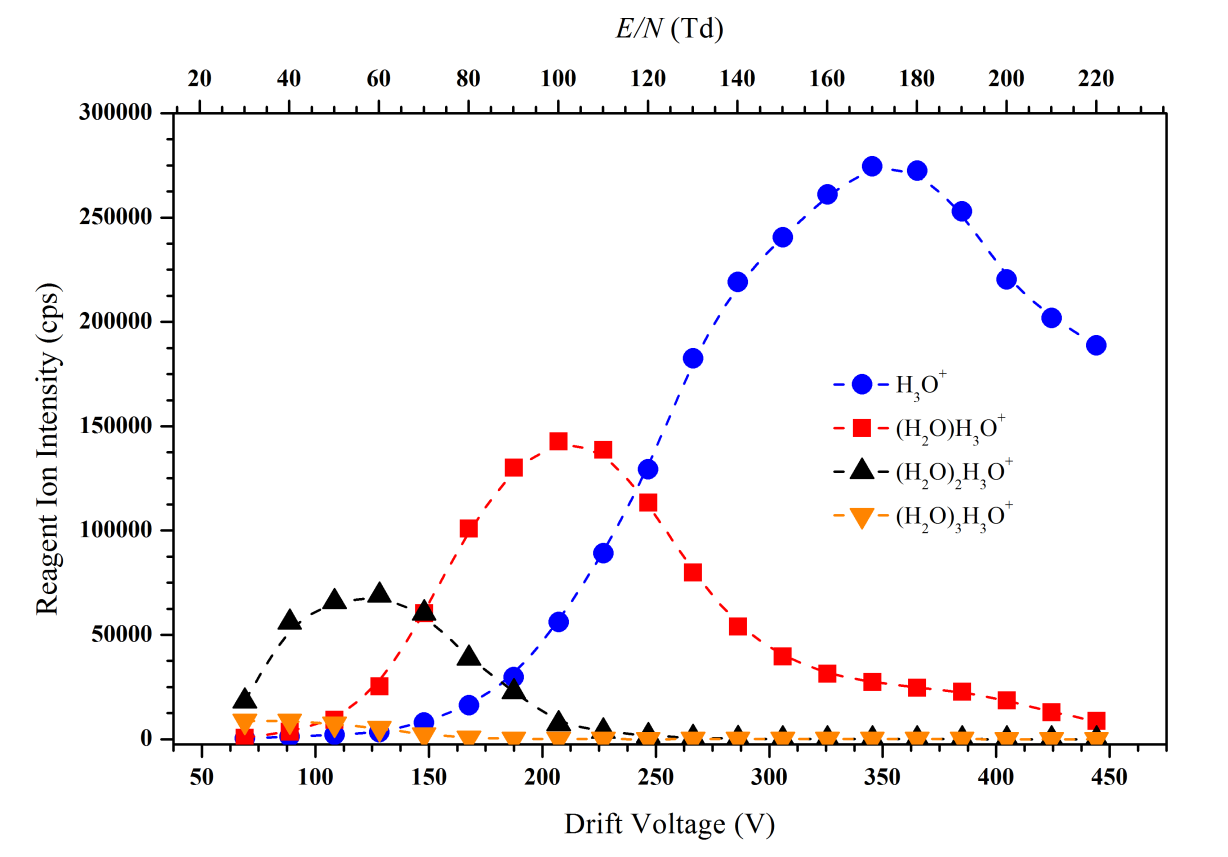
\includegraphics[width=0.60\linewidth]{pics/ISOF/ANAESTH_004.png}
}

\sidesubfloat[]{
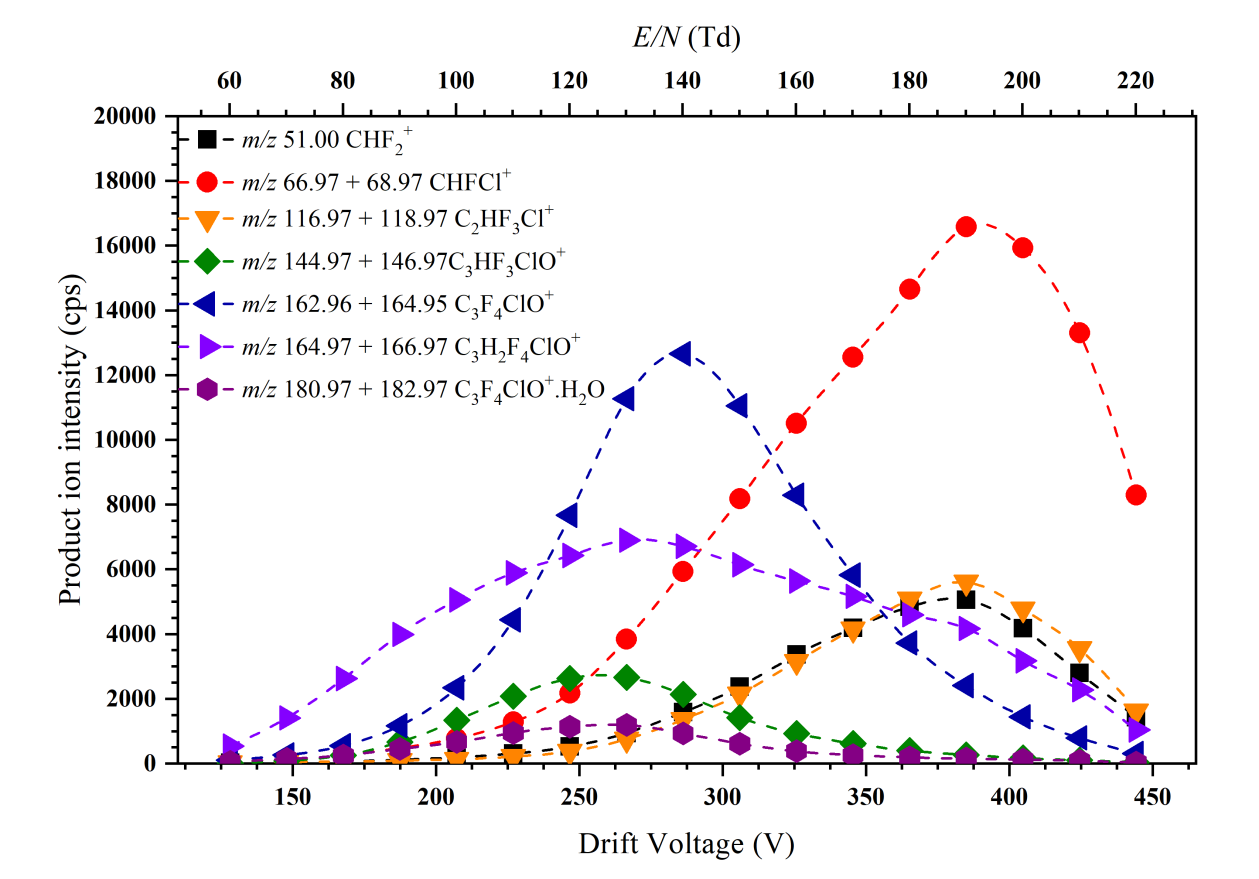
\includegraphics[width=0.60\linewidth]{pics/ISOF/ANAESTH_006.png}
}

\sidesubfloat[]{
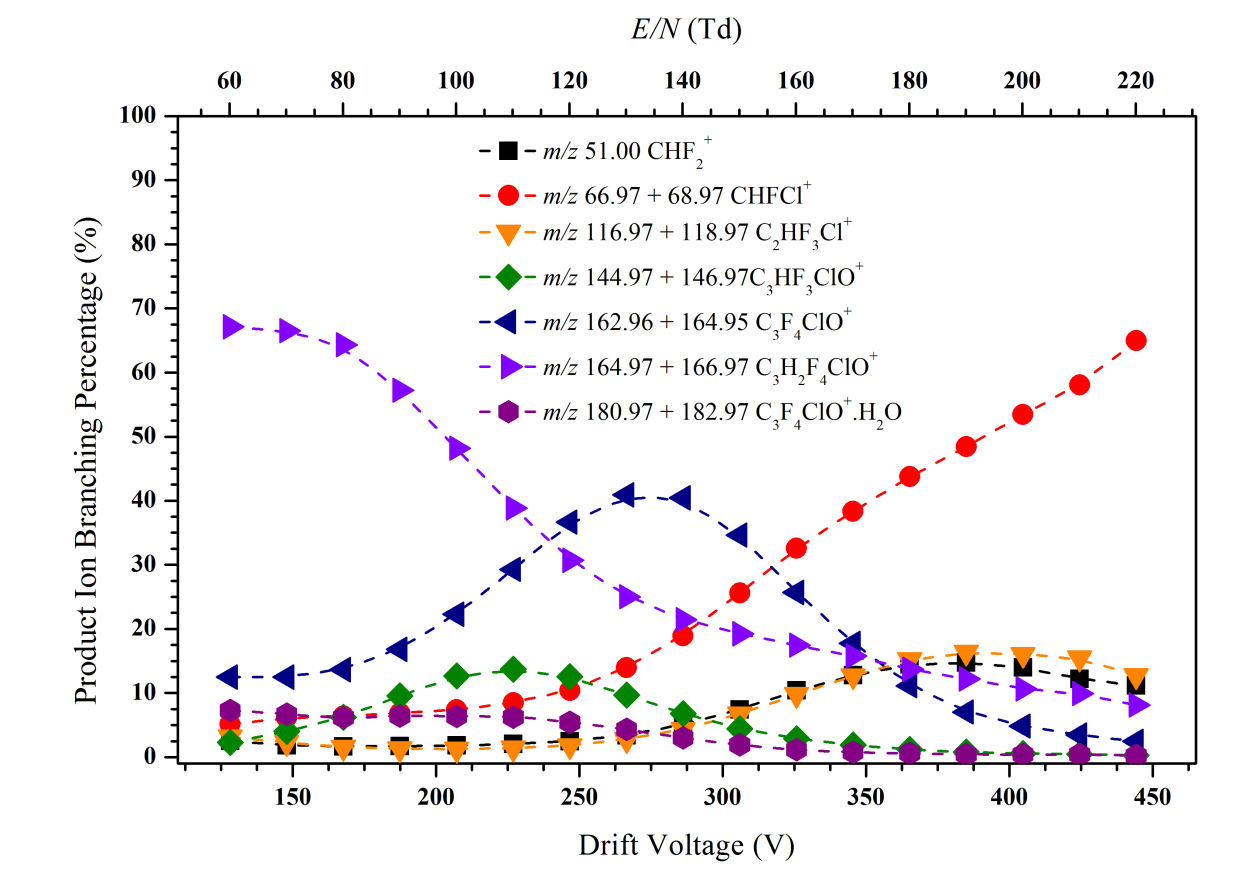
\includegraphics[width=0.60\linewidth]{pics/ISOF/ANAESTH_005.png}
}

\caption{(a) Reagent ions intensity plot and product ions  (b) intensity and (c) distribution plots from the reaction of isoflurane and (H$_2$O)$_n$H$_3$O$^+$ in humid conditions.}
\label{fig:isof_h3o_h}
\end{figure}

%\subsubsection{Isoflurane: charge transfer mode}

\begin{figure}%[h]
\centering
\sidesubfloat[]{
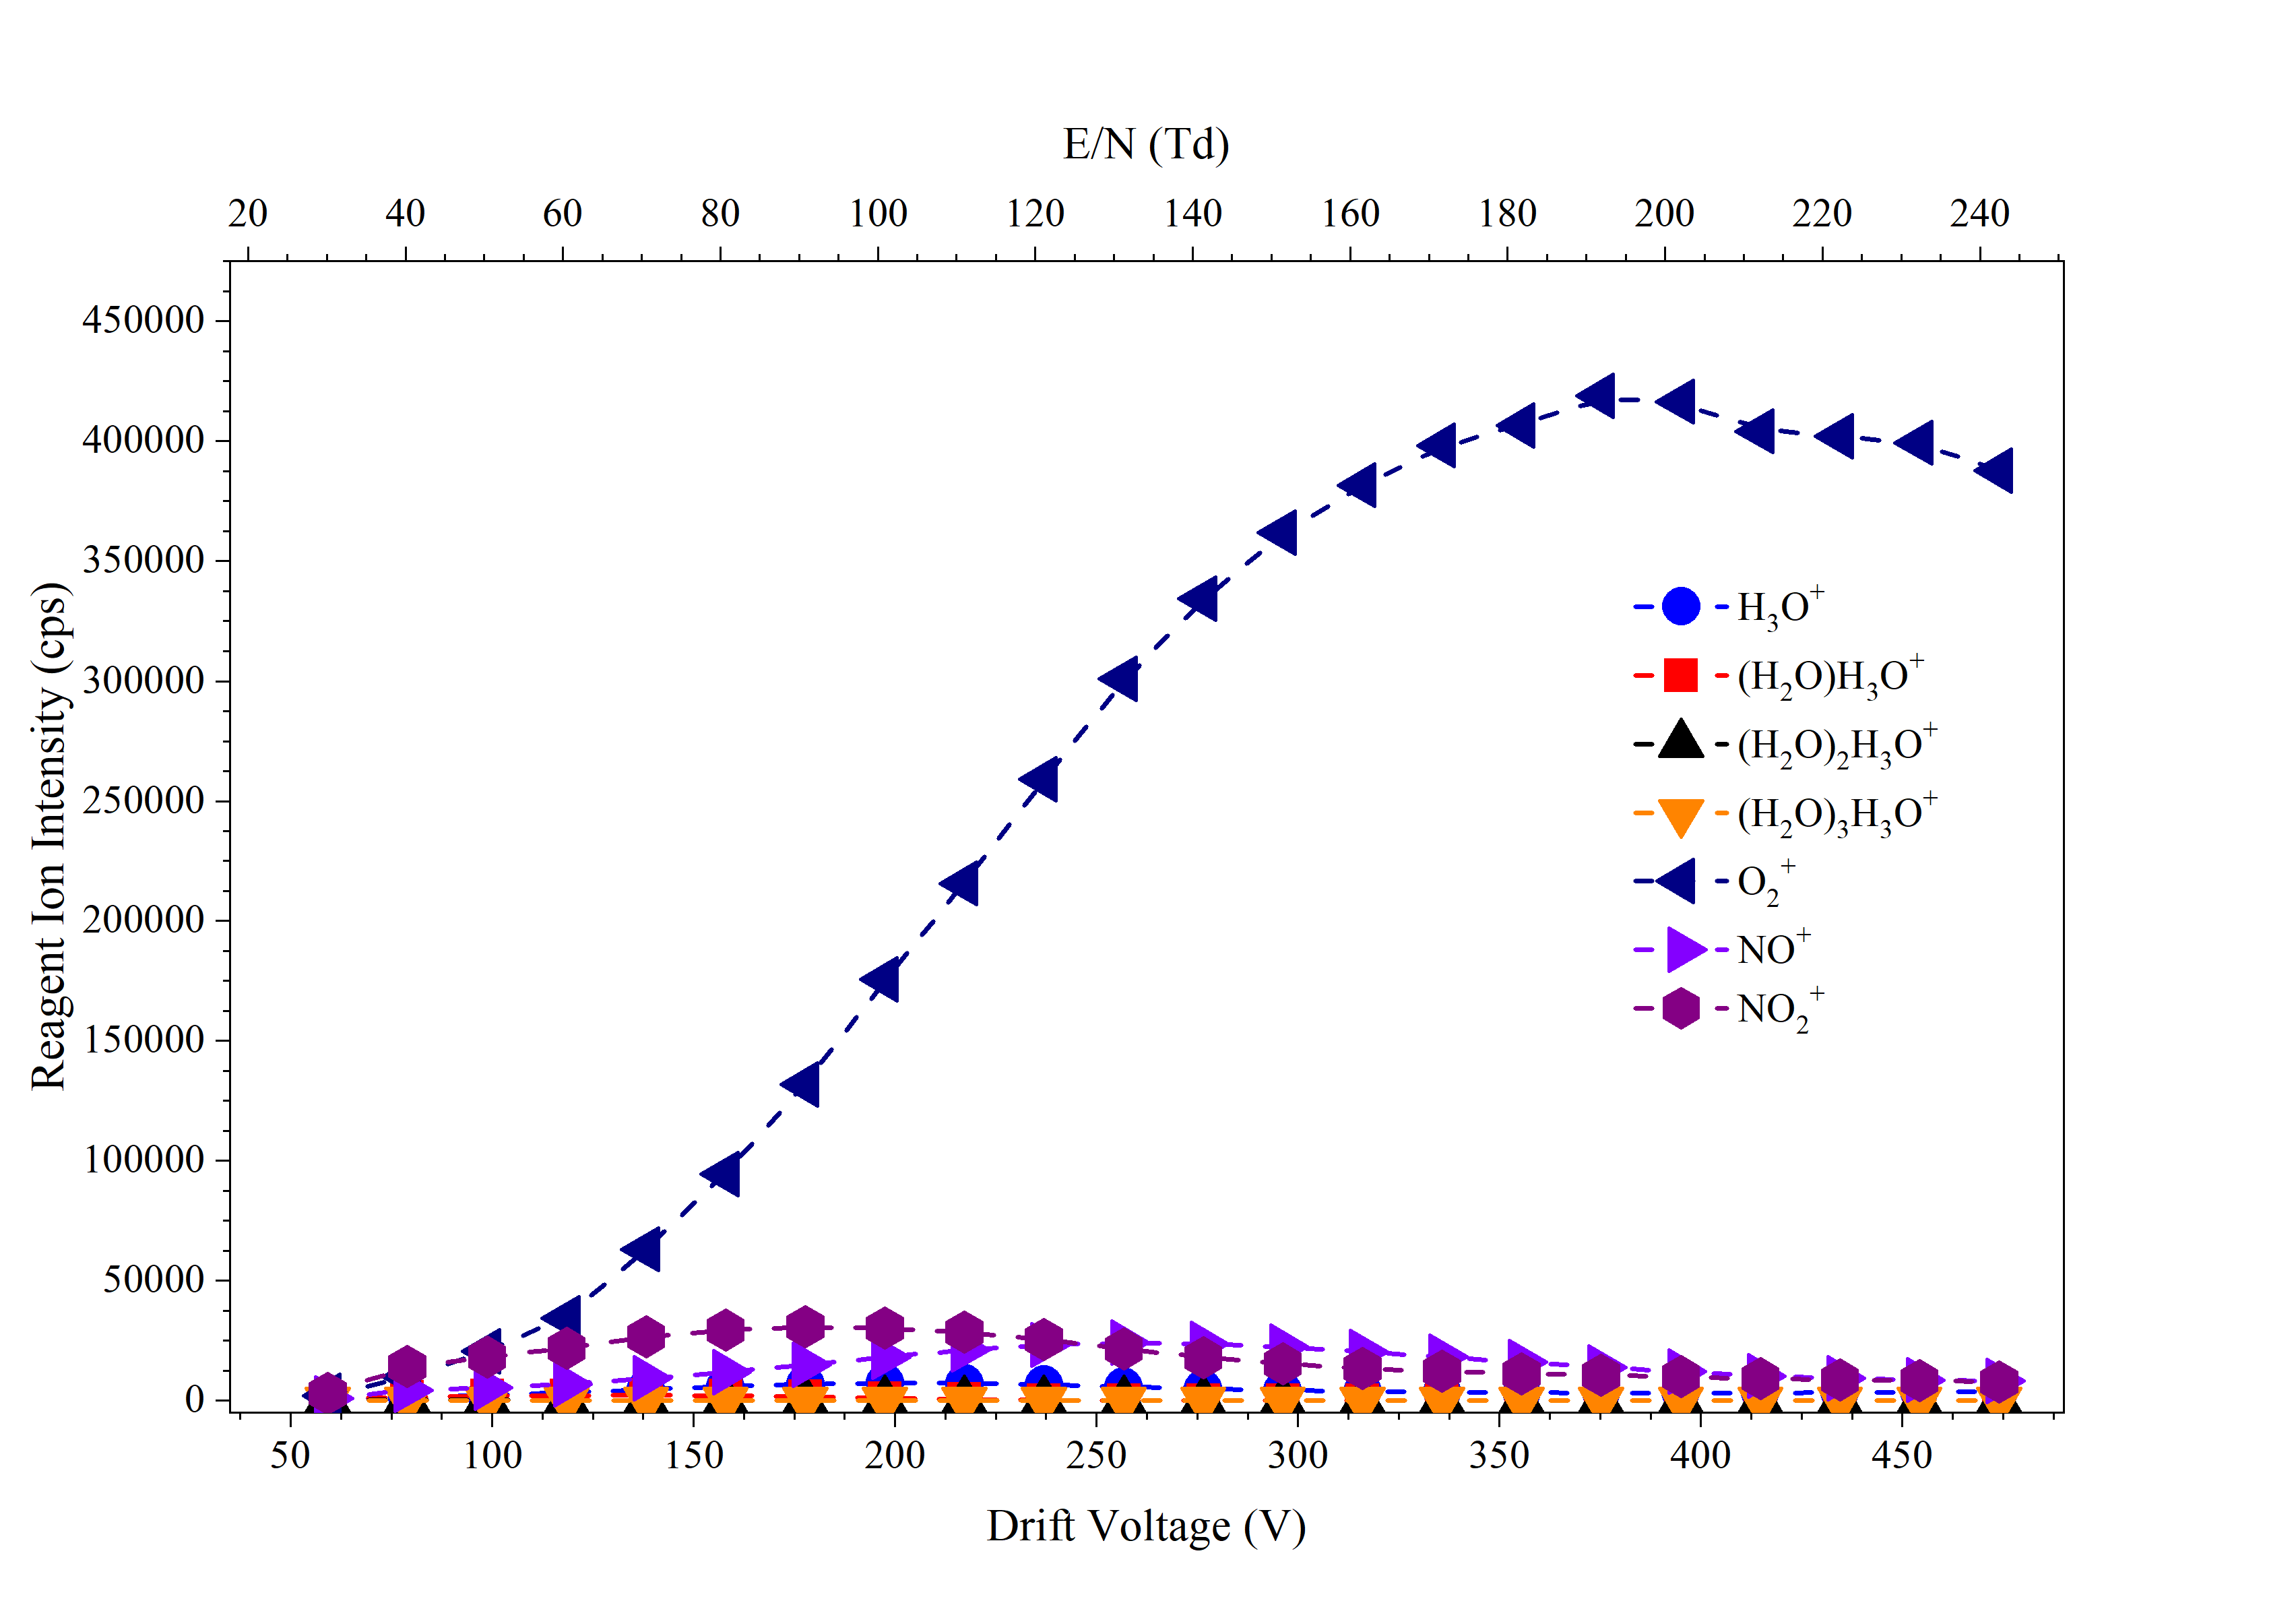
\includegraphics[width=0.60\linewidth]{pics/RIdryISOFo2.png}
}

\sidesubfloat[]{
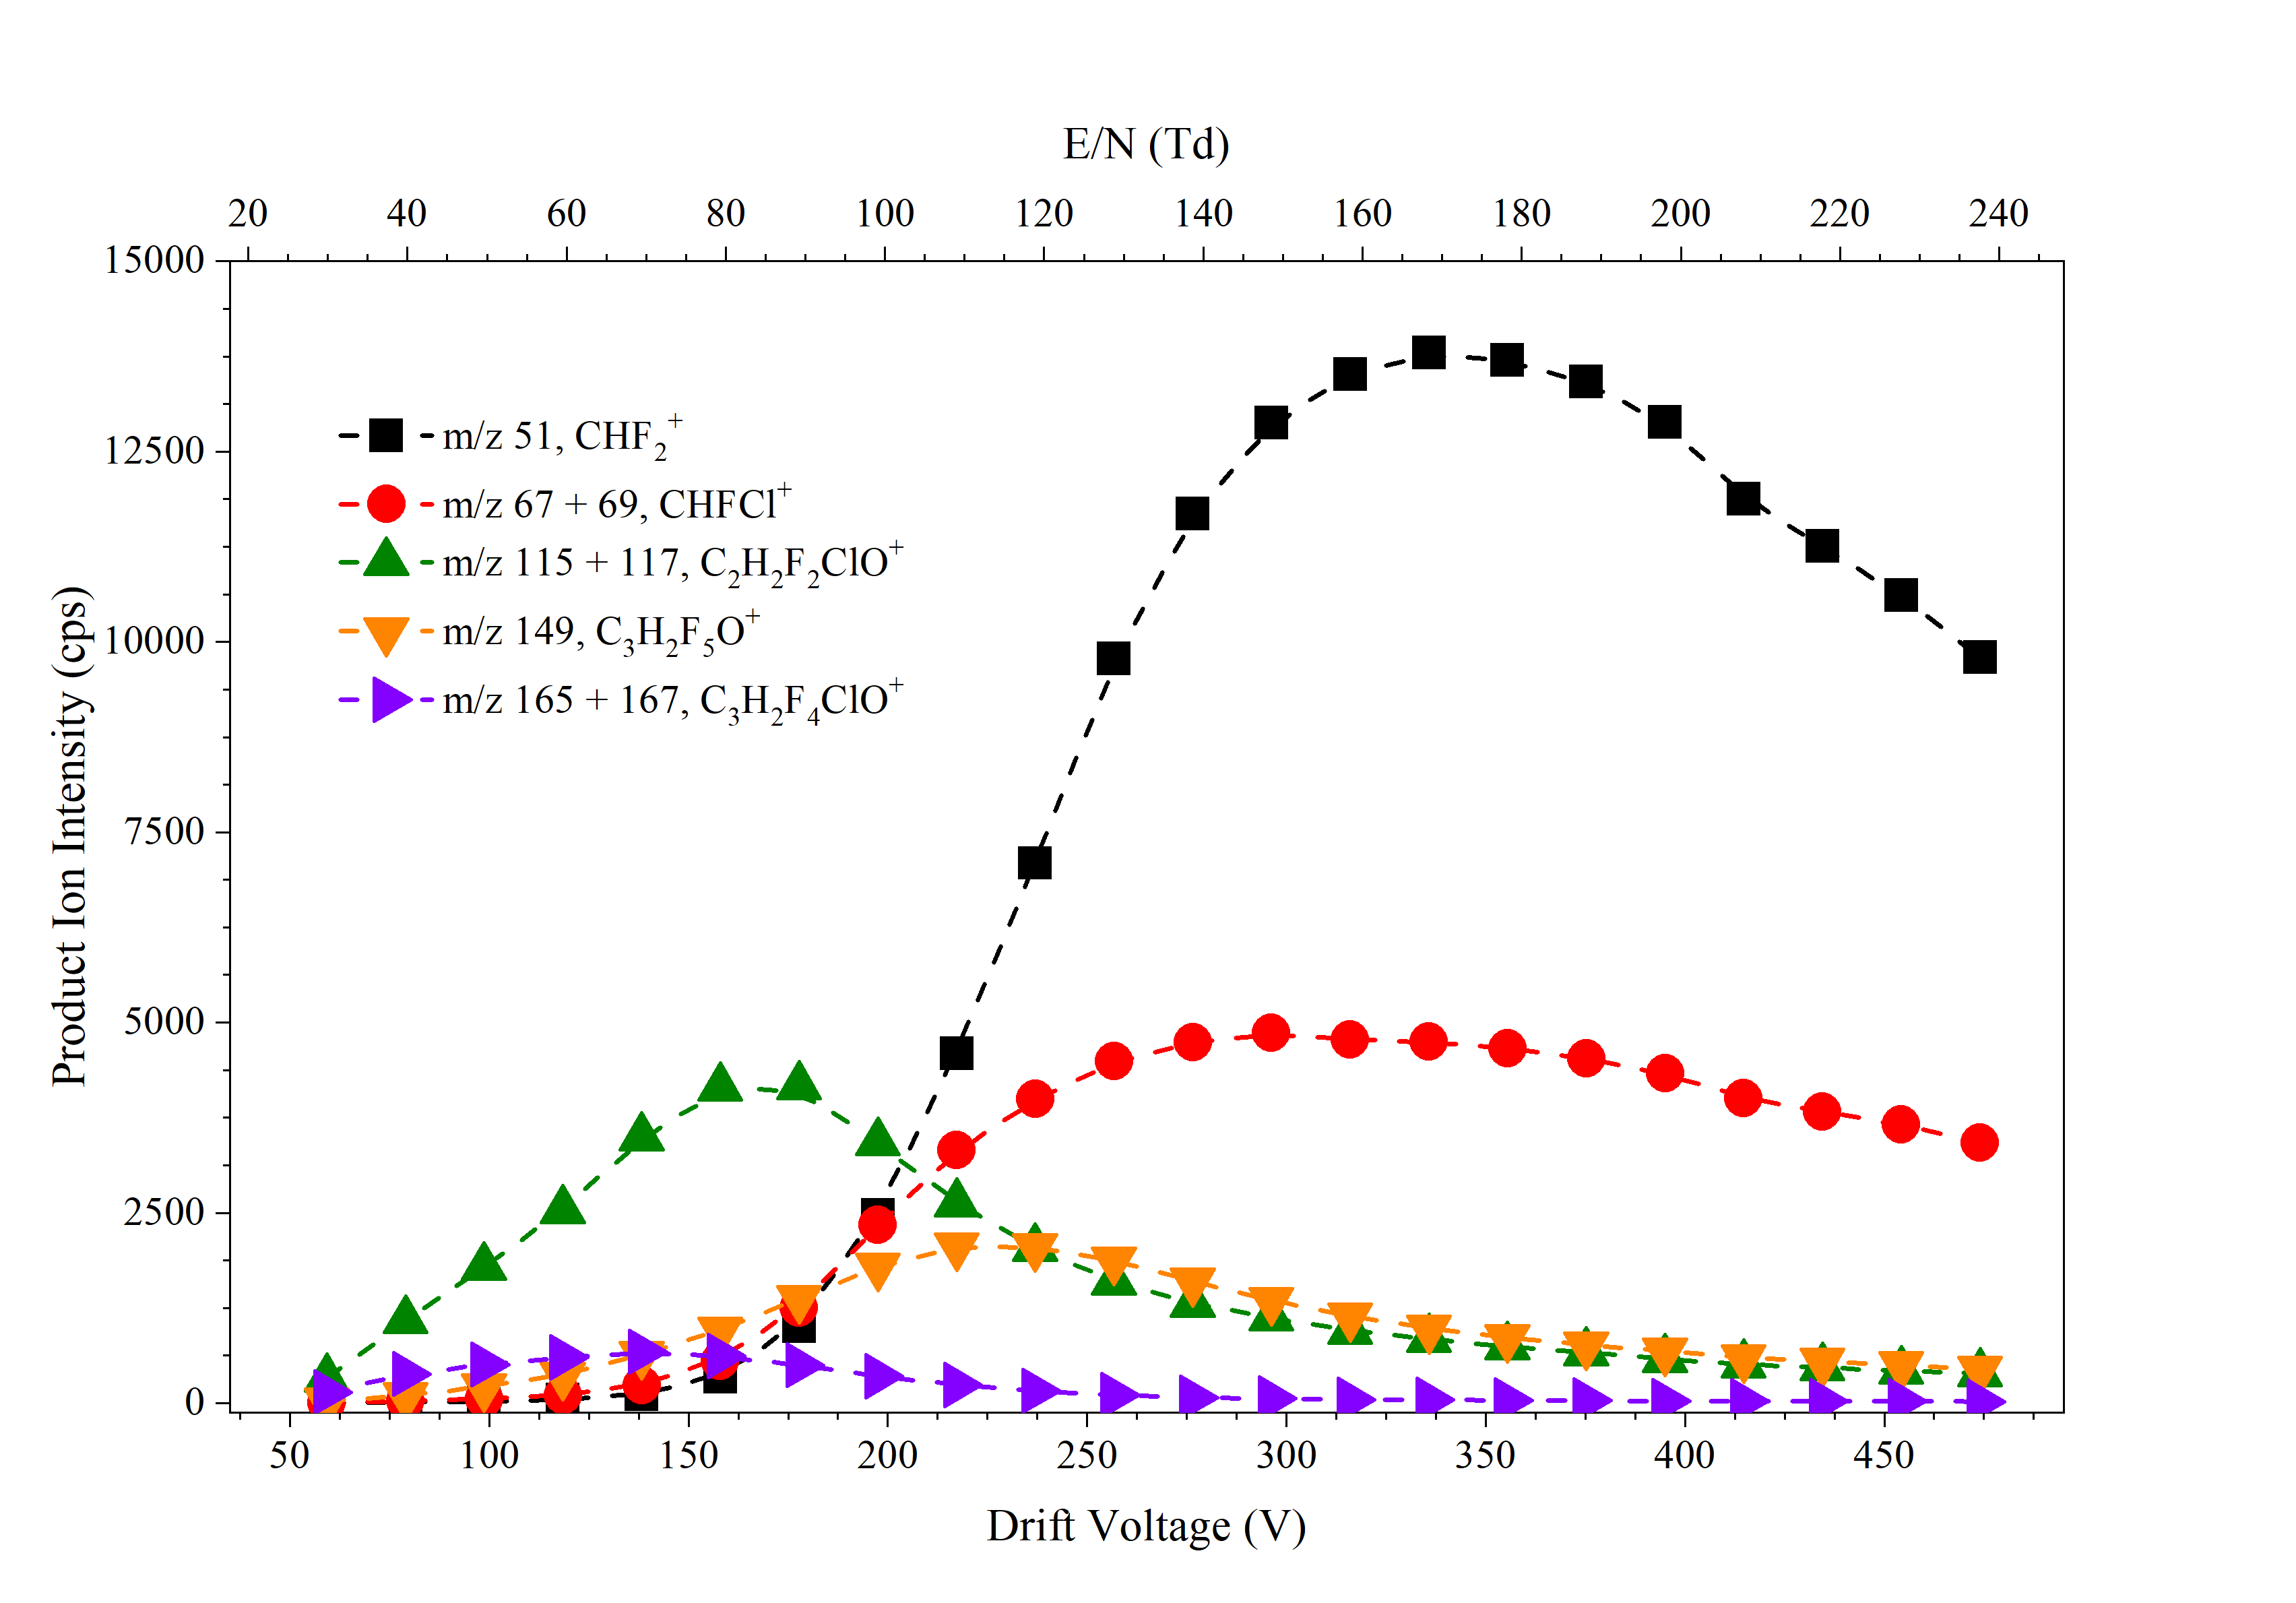
\includegraphics[width=0.60\linewidth]{pics/ISOFo2DRY.png}
}

\sidesubfloat[]{
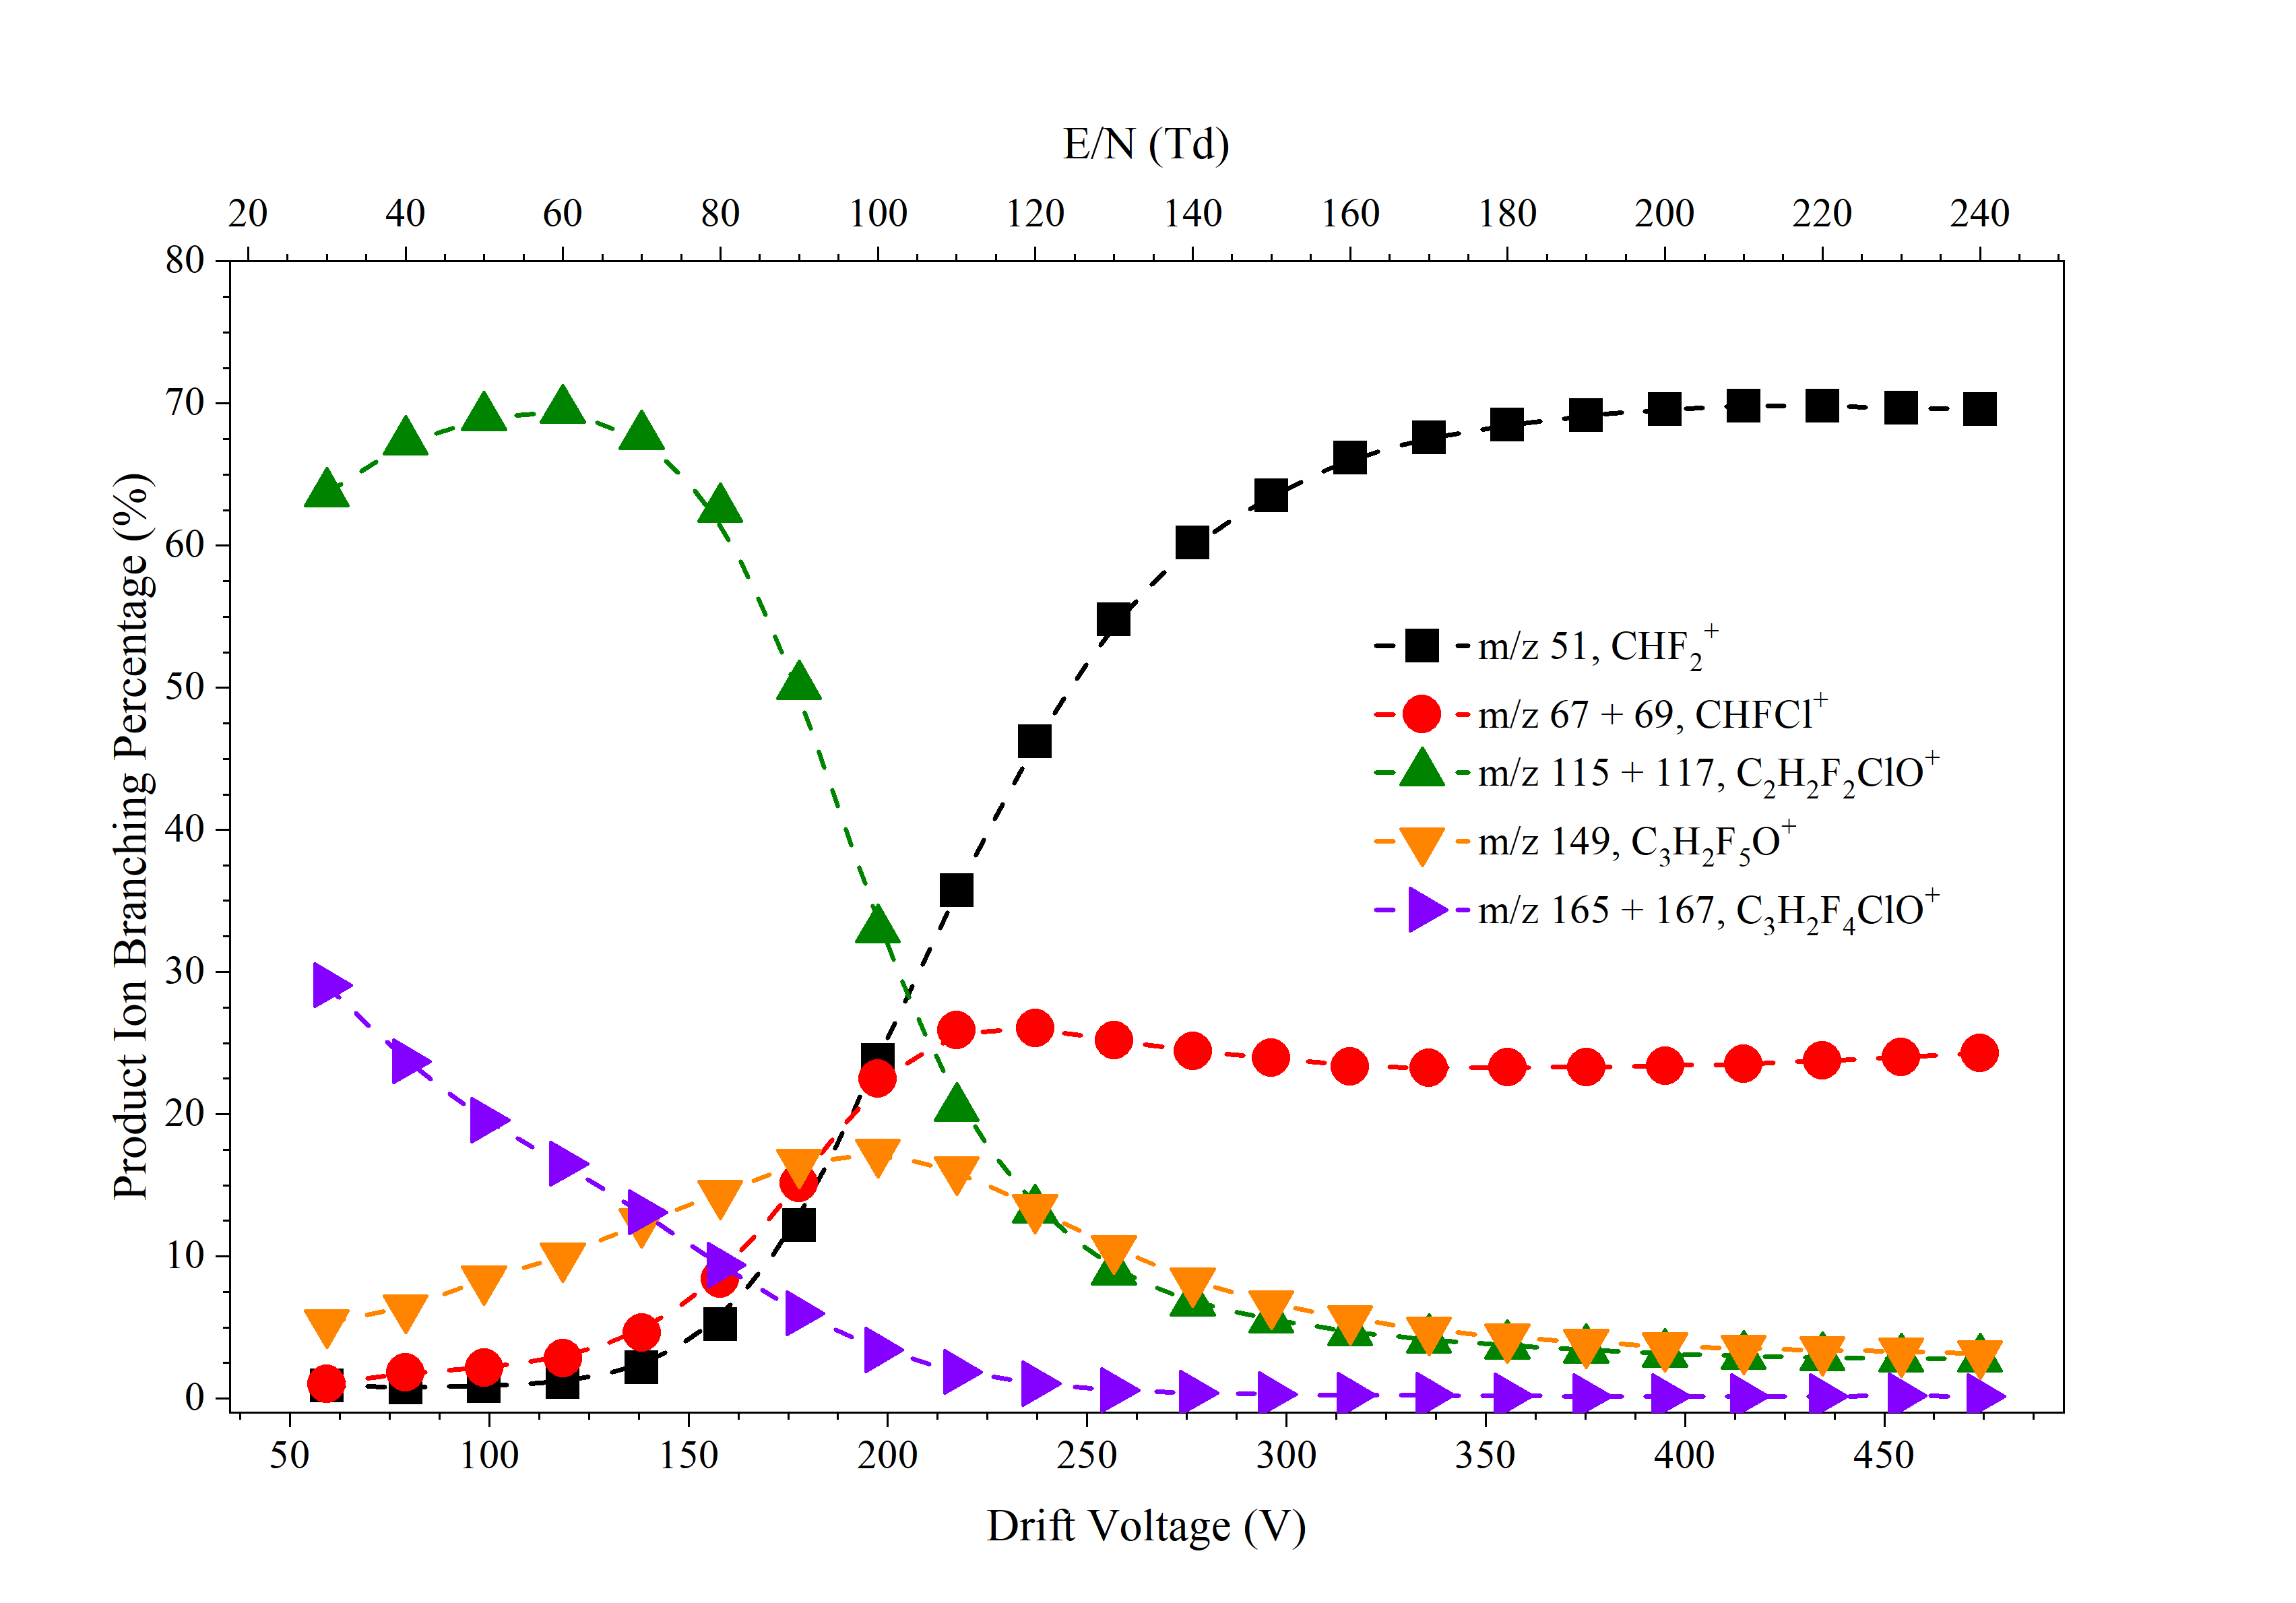
\includegraphics[width=0.60\linewidth]{pics/ISOFo2DRY-BR.png}
}
\caption{(a) Reagent ions intensity plot and product ions  (b) intensity and (c) distribution plots from the reaction of isoflurane and O$_2^+$ in dry conditions.}
\label{fig:isof_o2}
\end{figure}

\begin{figure}%[h]
\centering
\sidesubfloat[]{
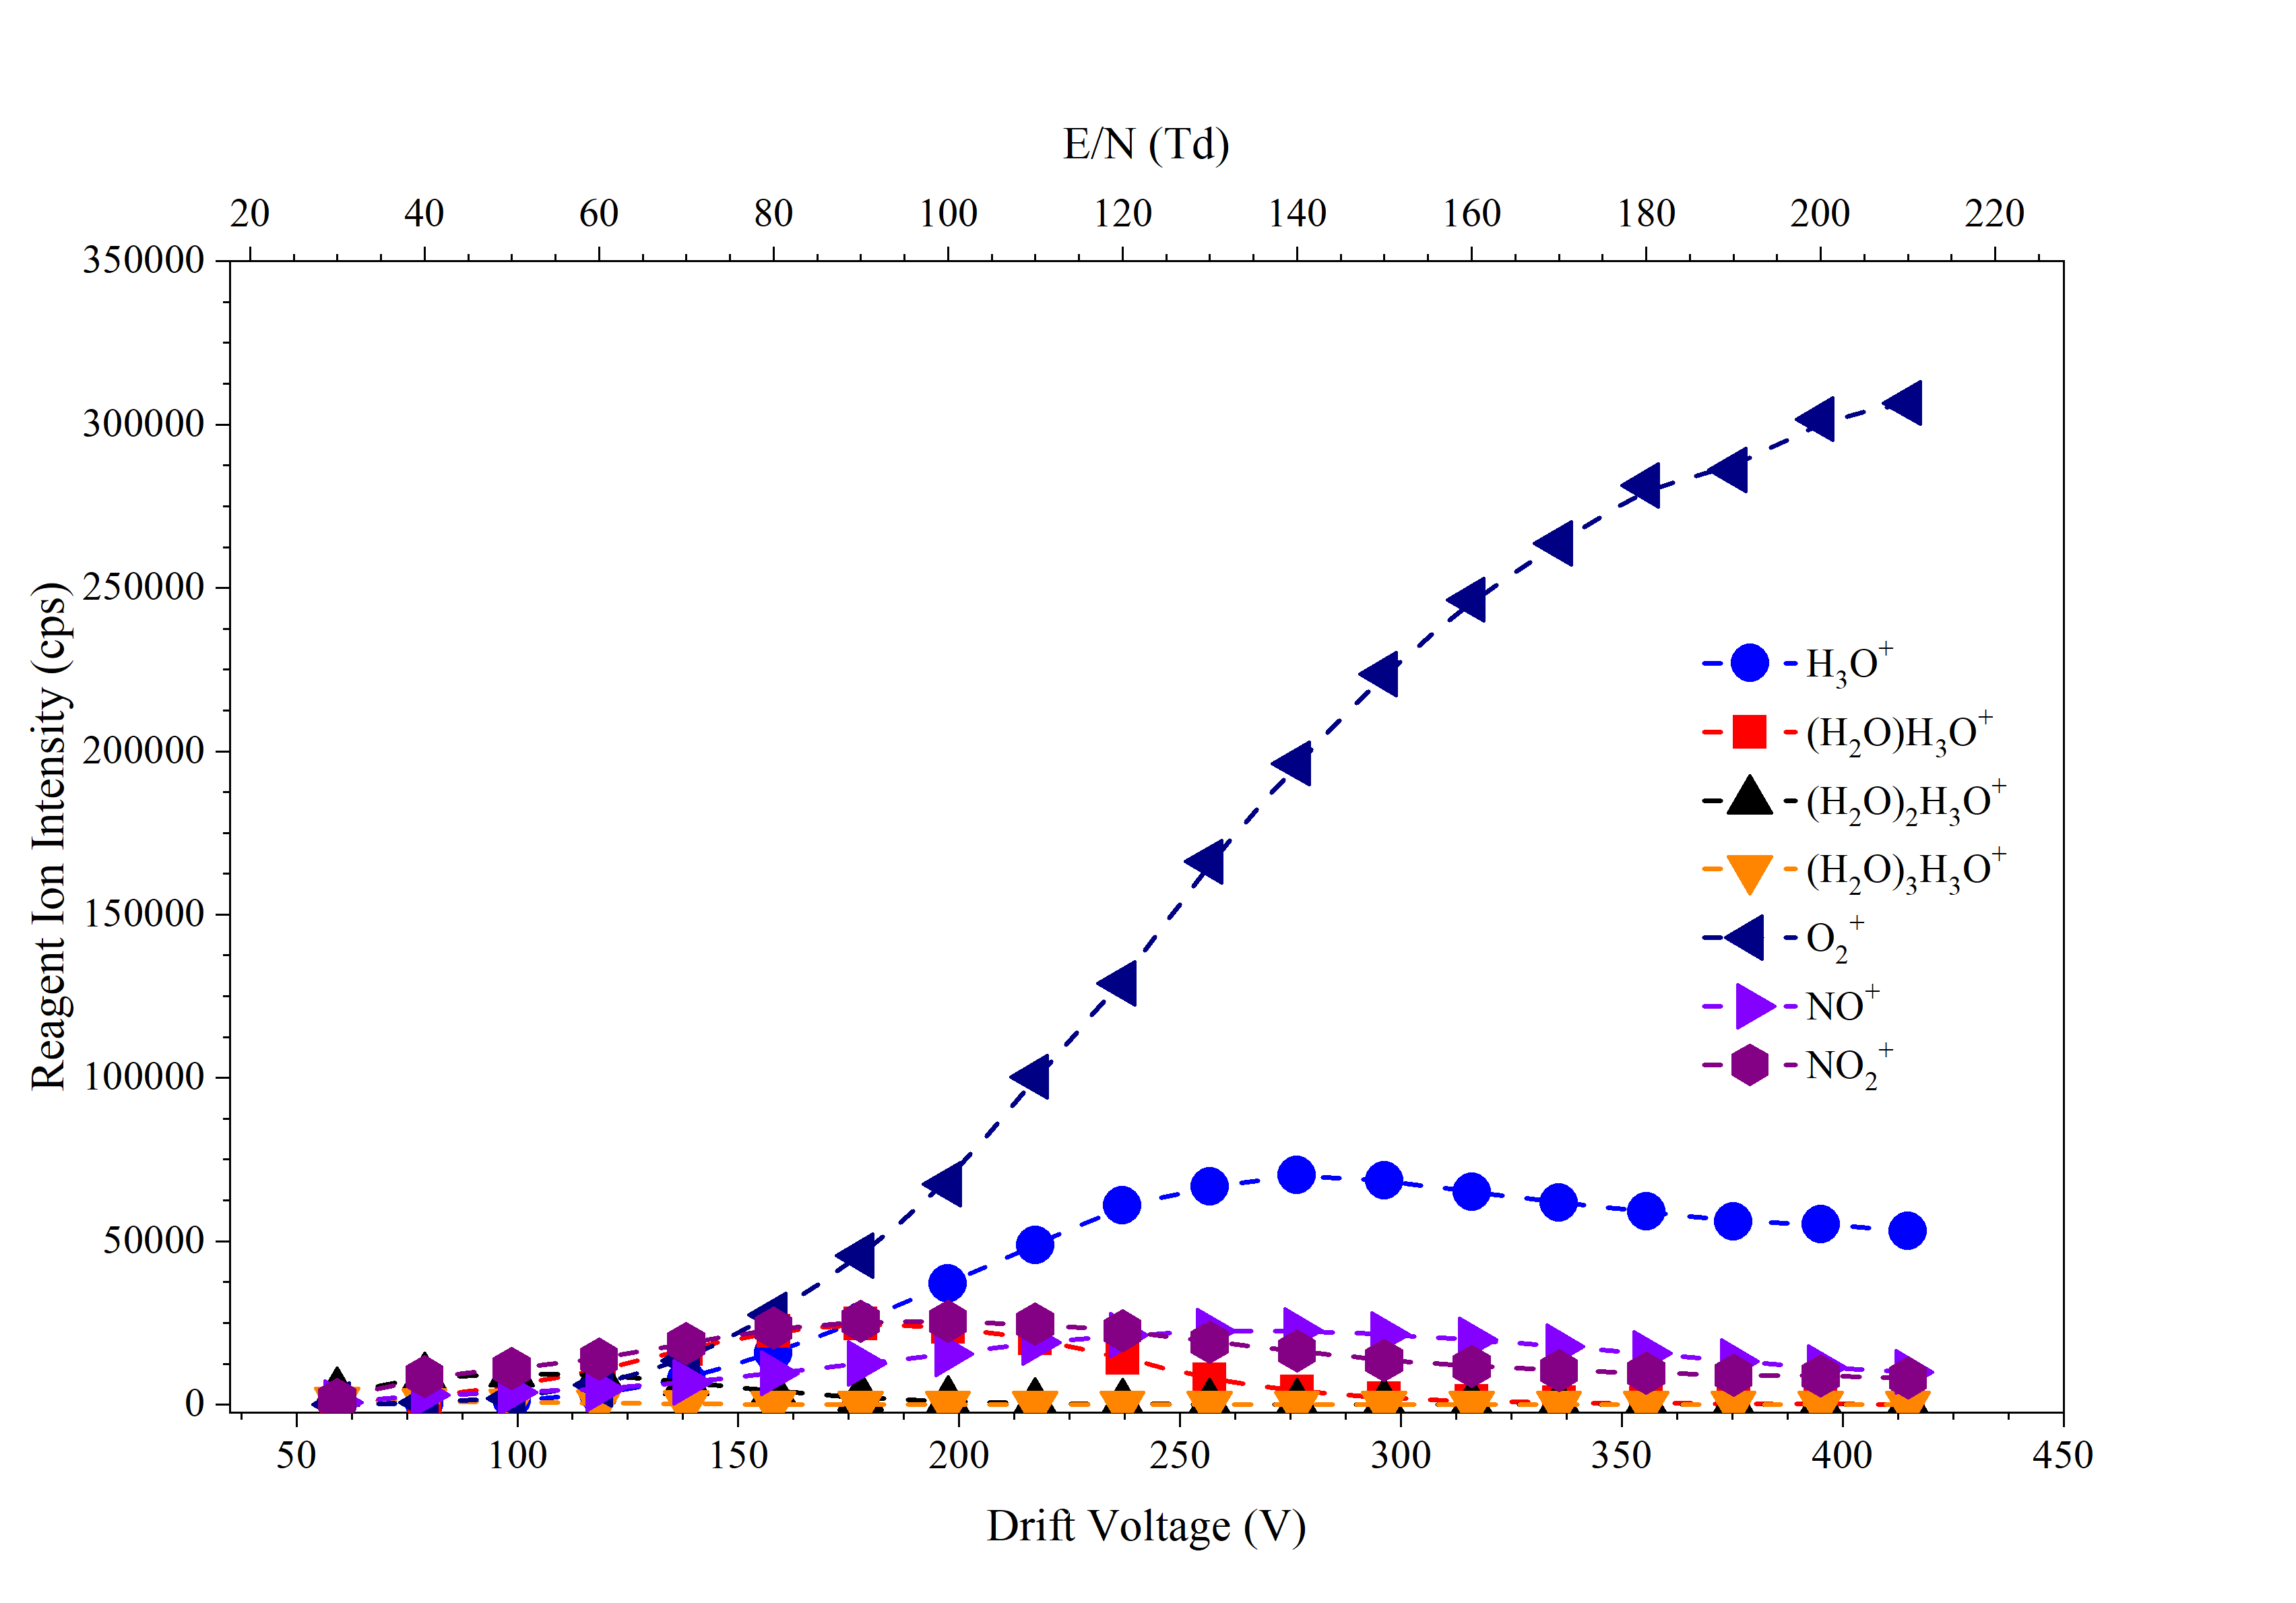
\includegraphics[width=0.60\linewidth]{pics/RIhumidISOFo2.png}
}

\sidesubfloat[]{
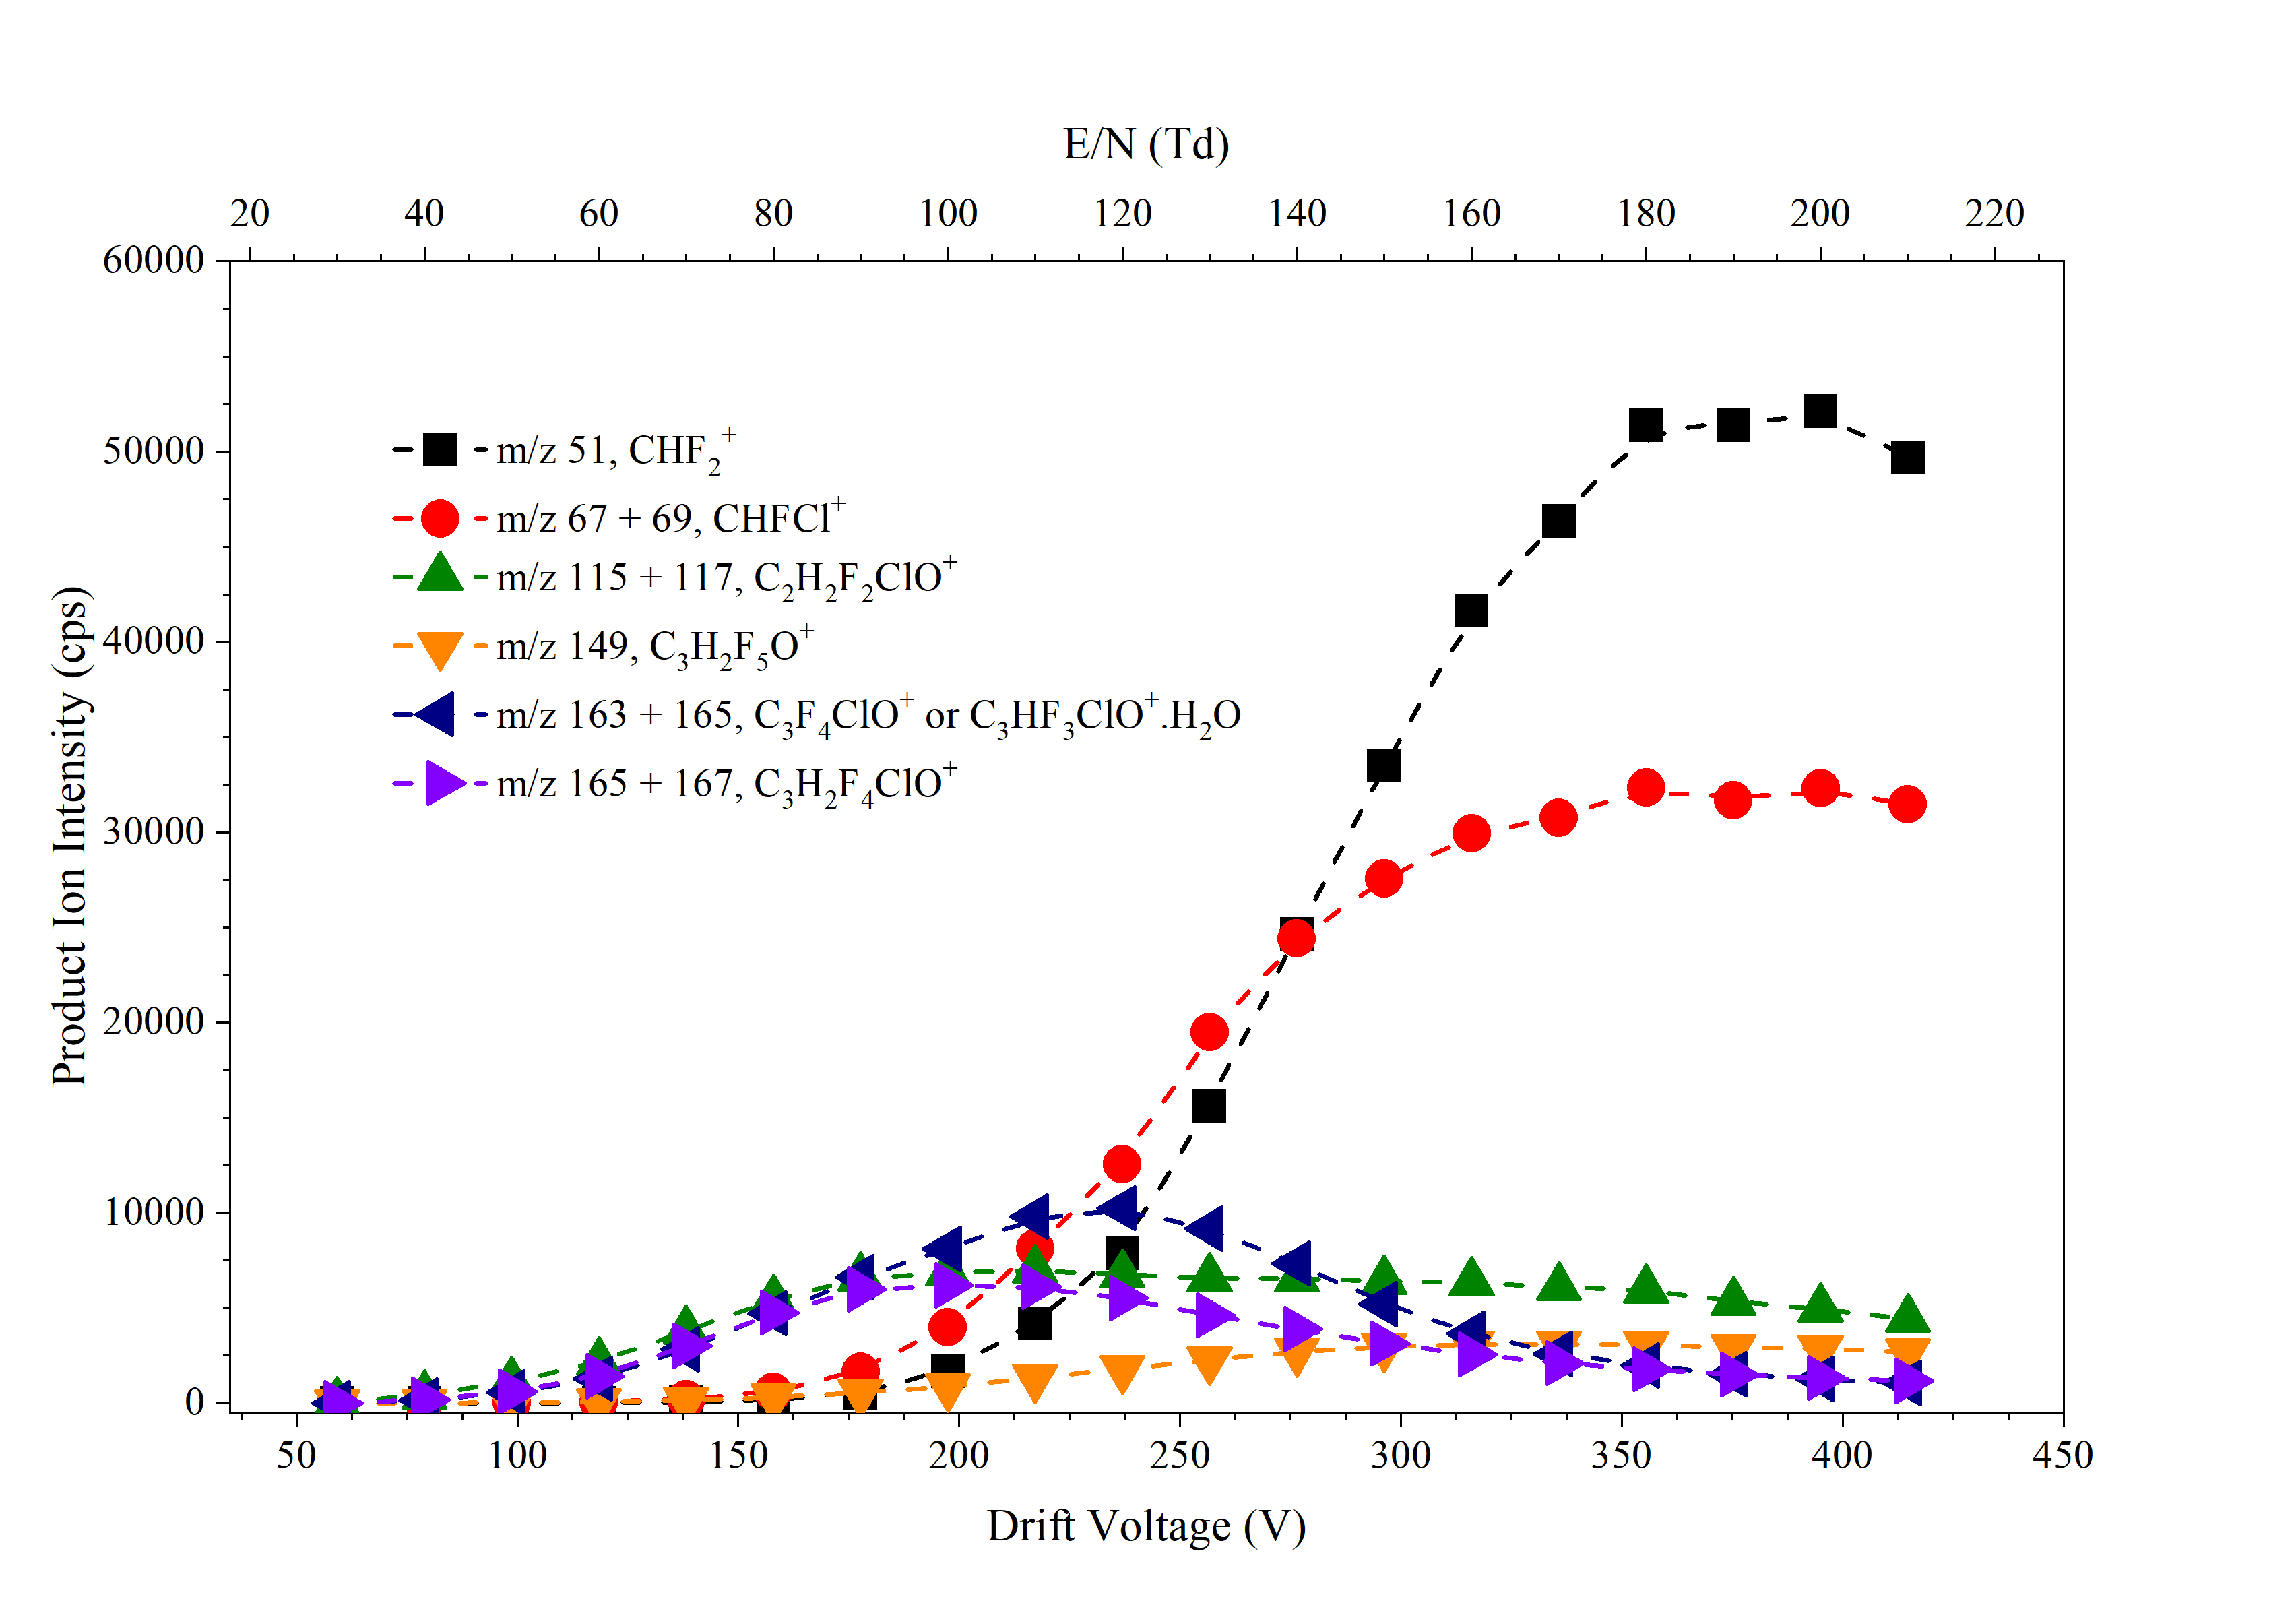
\includegraphics[width=0.60\linewidth]{pics/ISOFo2HUMID.png}
}

\sidesubfloat[]{
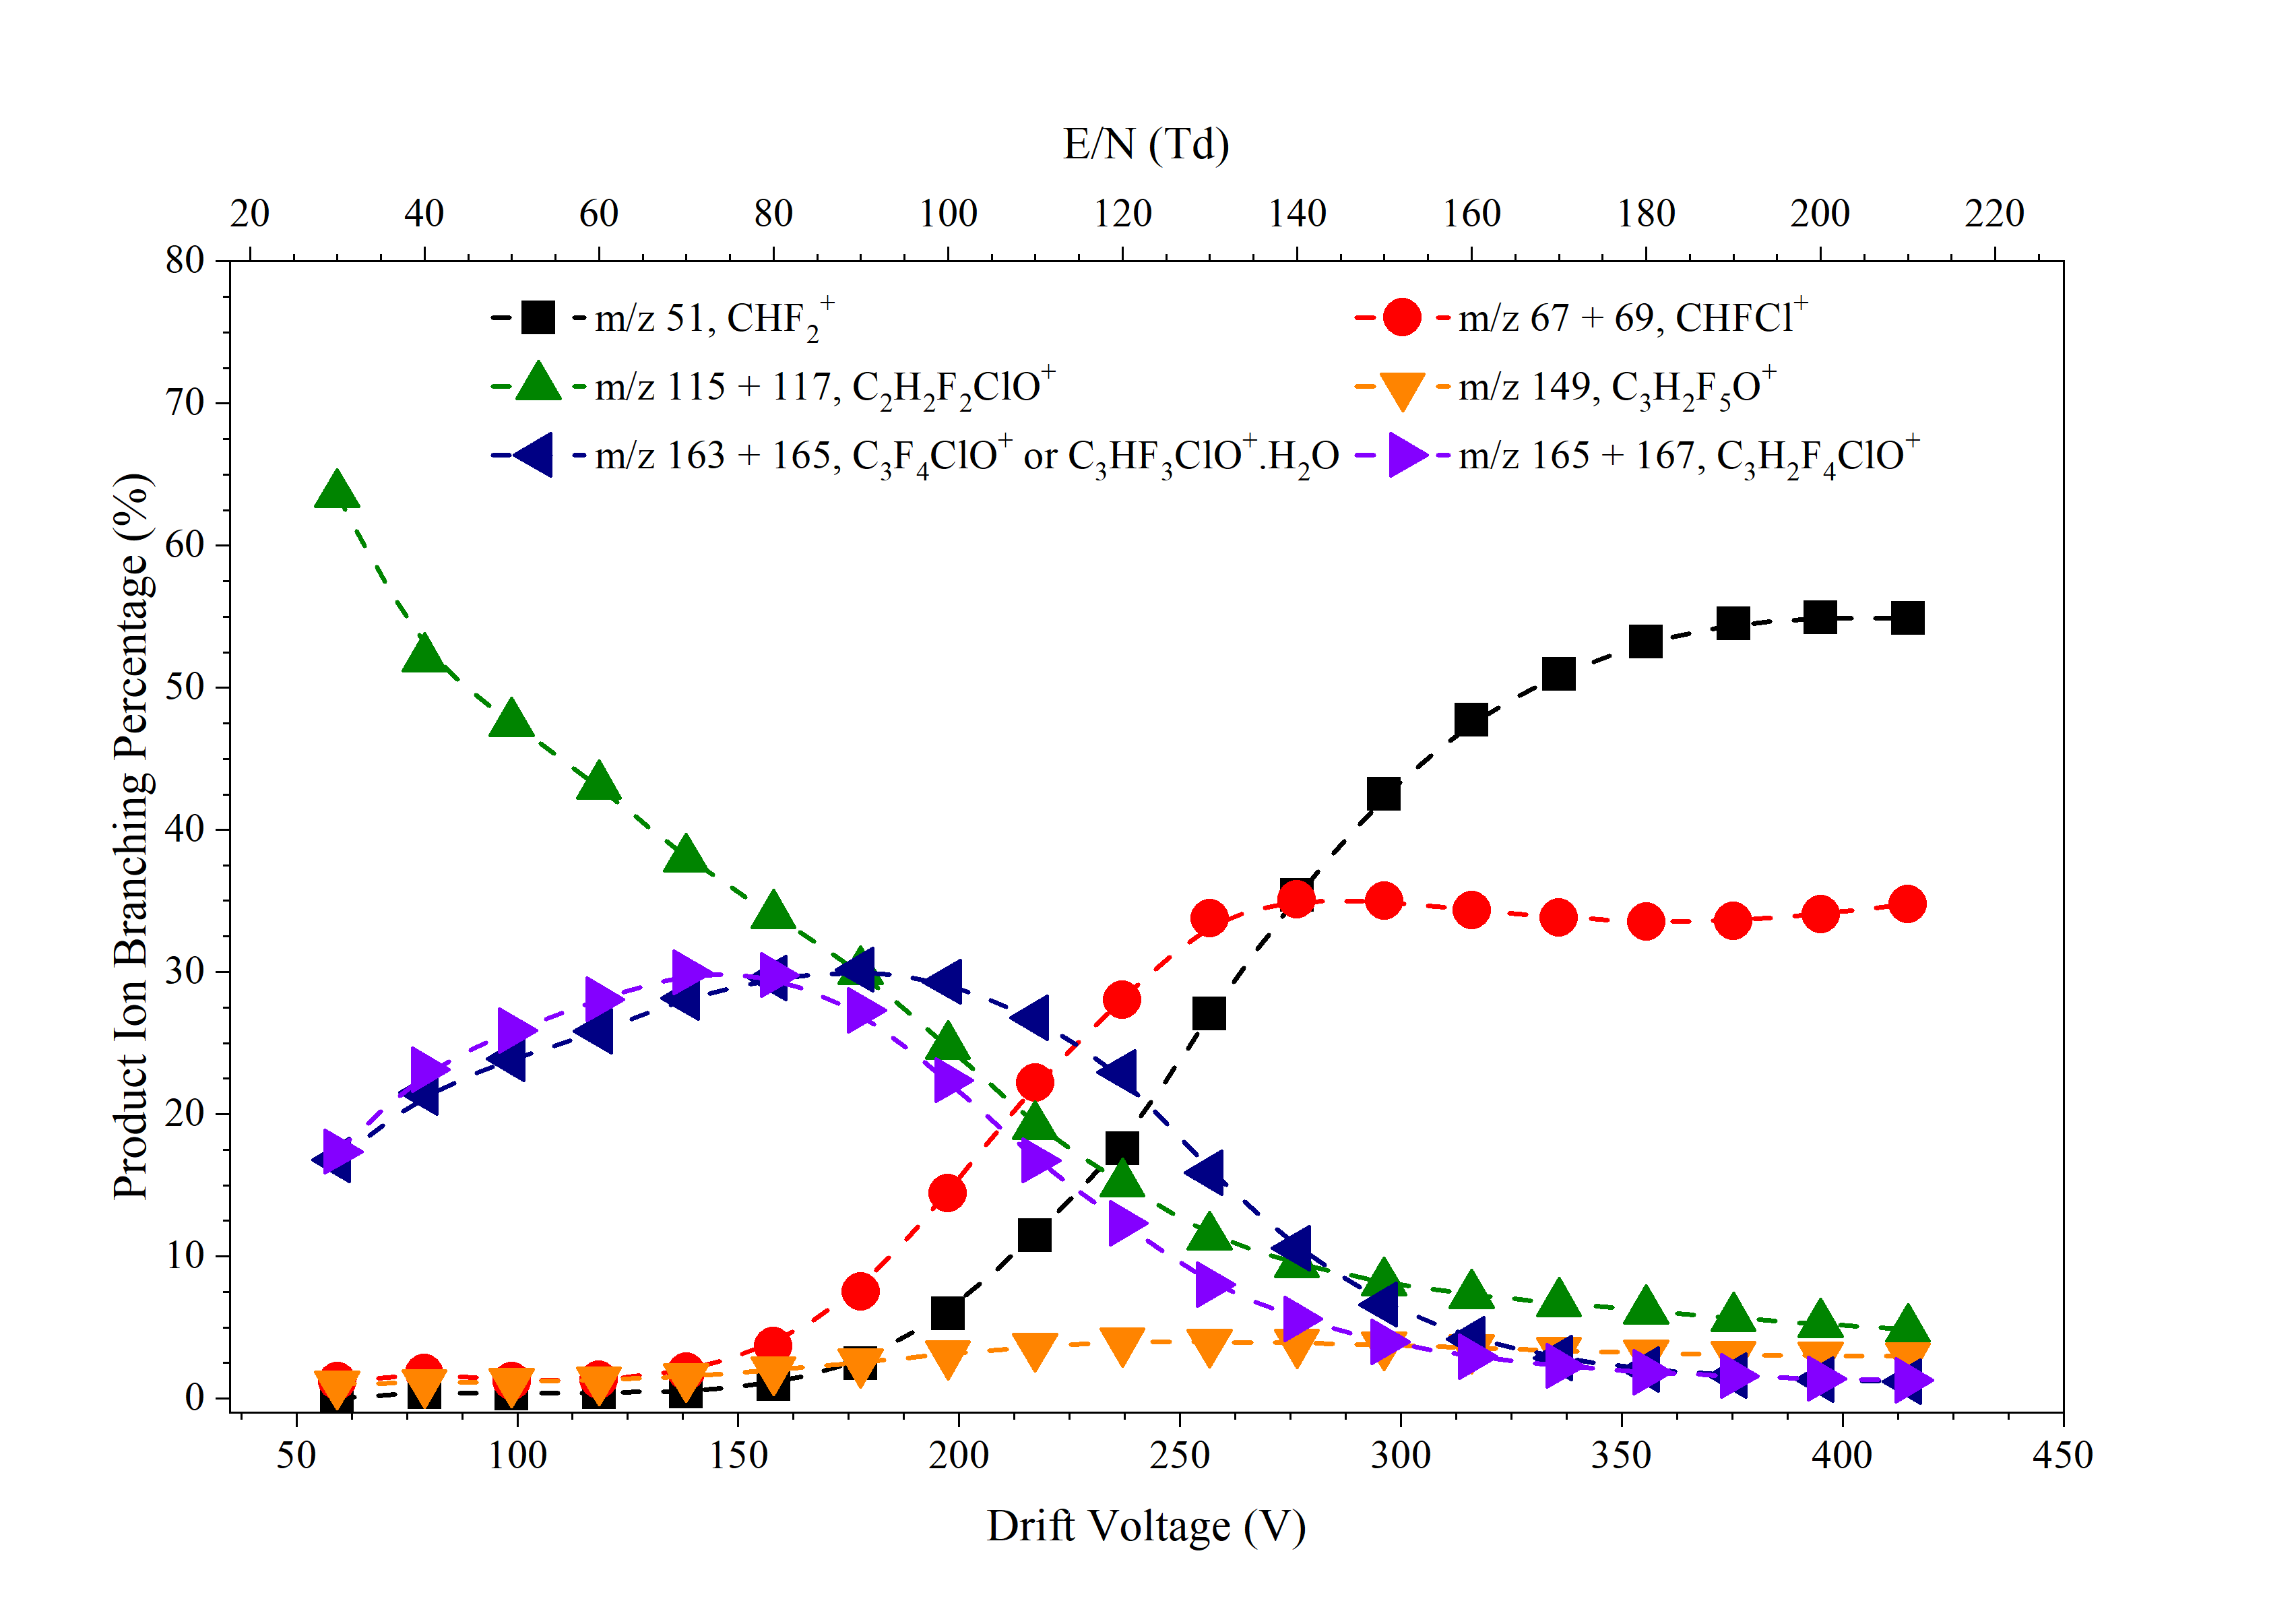
\includegraphics[width=0.60\linewidth]{pics/ISOFo2HUMID-BR.png}
}
\caption{(a) Reagent ions intensity plot and product ions  (b) intensity and (c) distribution plots from the reaction of isoflurane and O$_2^+$ in humid conditions.}
\label{fig:isof_o2_h}
\end{figure}


%\subsubsection{Sevoflurane: proton transfer mode}


\begin{figure}%[h]
\centering
\sidesubfloat[]{
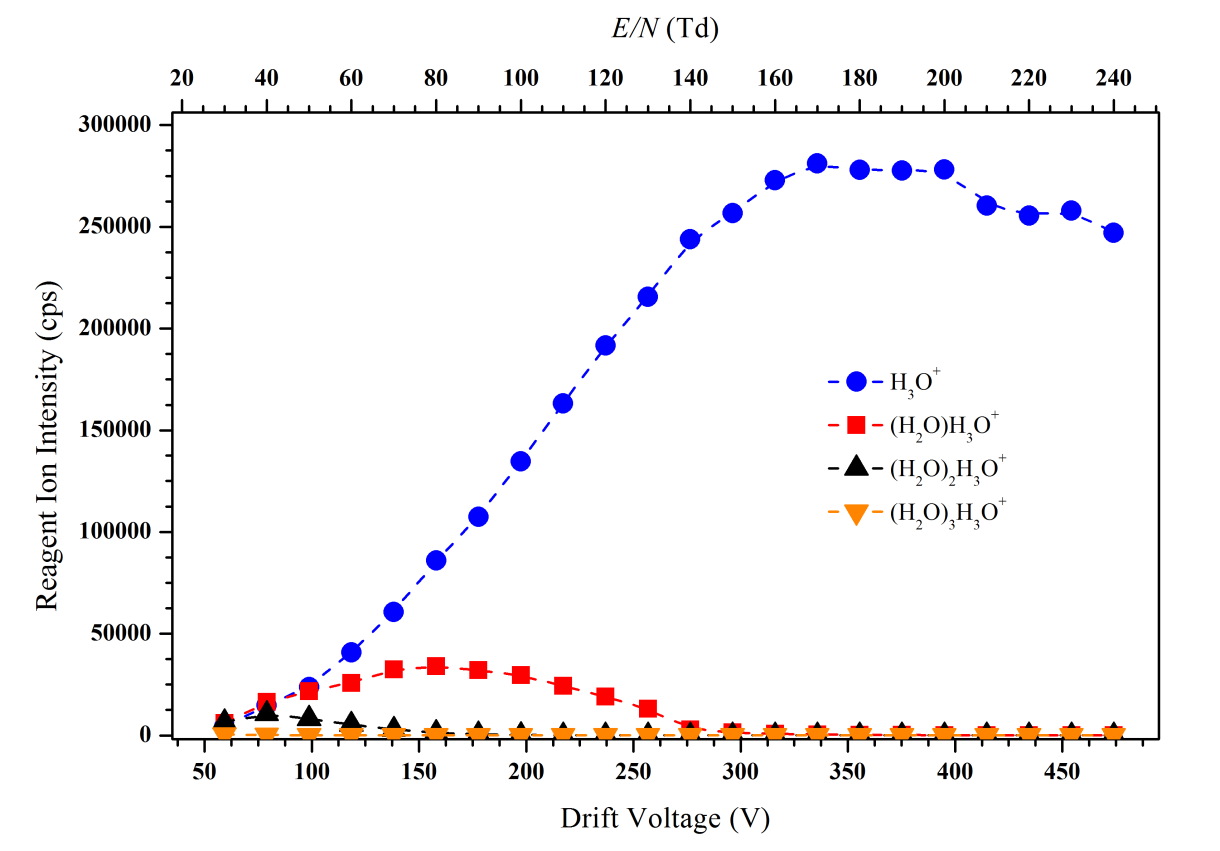
\includegraphics[width=0.60\linewidth]{pics/ISOF/ANAESTH_010.png}
}

\sidesubfloat[]{
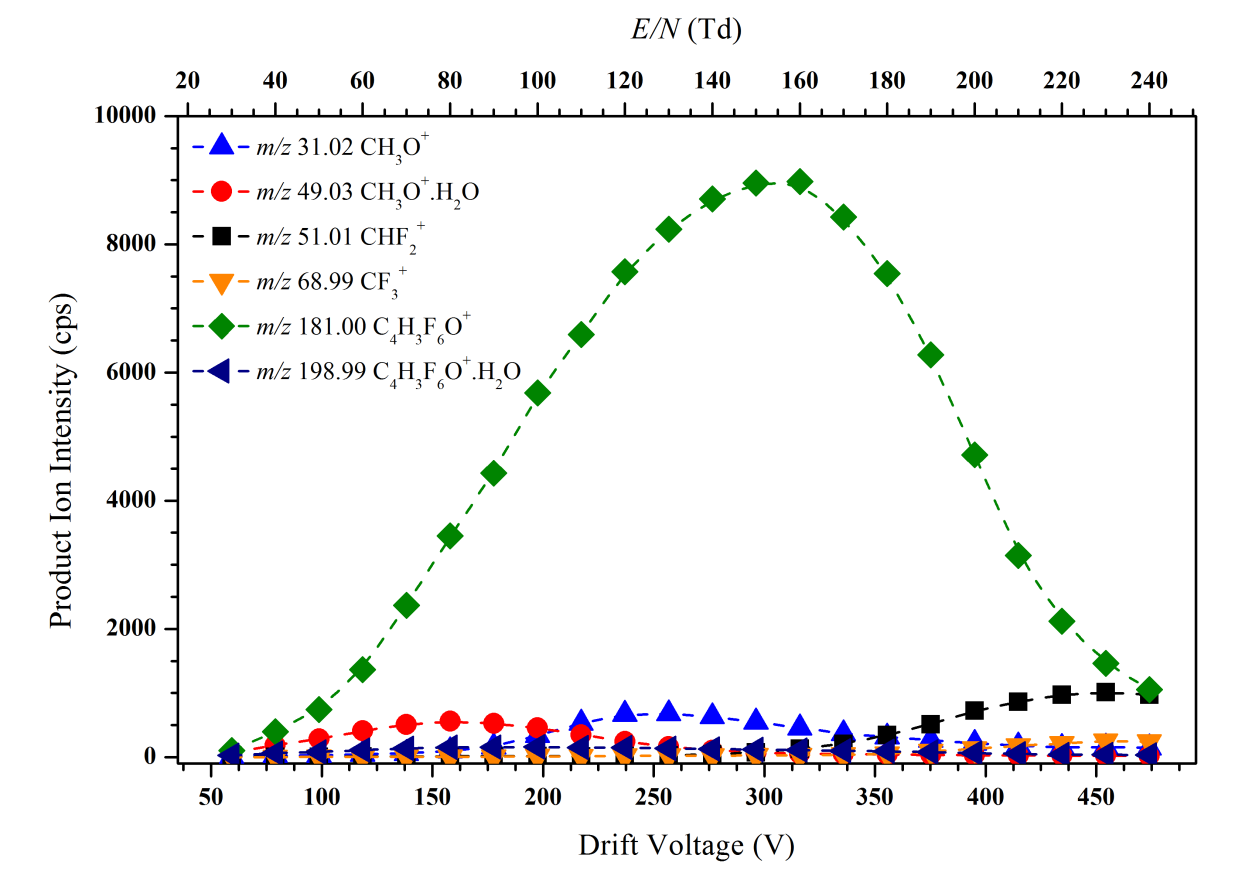
\includegraphics[width=0.60\linewidth]{pics/ISOF/ANAESTH_014.png}
}

\sidesubfloat[]{
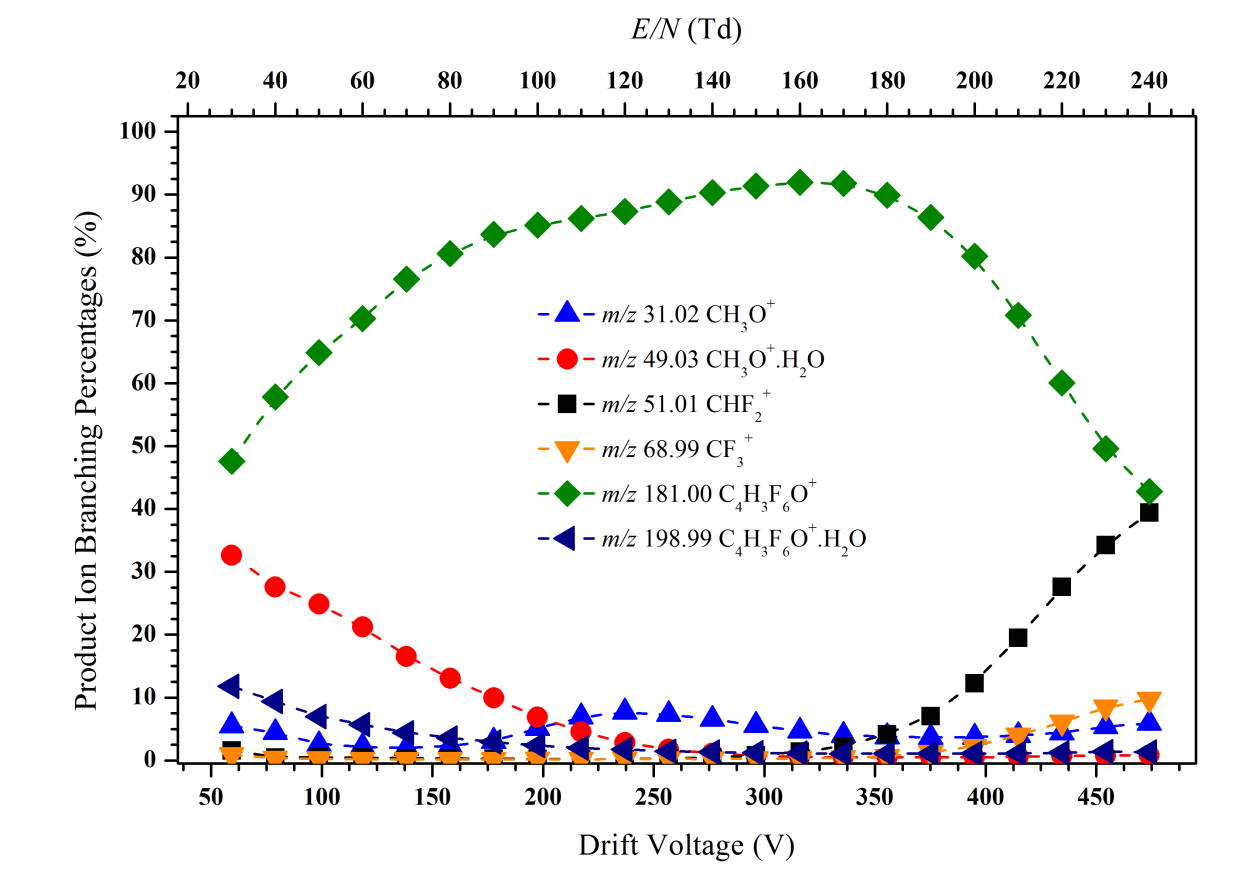
\includegraphics[width=0.60\linewidth]{pics/ISOF/ANAESTH_012.png}
}

\caption{(a) Reagent ions intensity plot and product ions  (b) intensity and (c) distribution plots from the reaction of sevoflurane and (H$_2$O)$_n$H$_3$O$^+$ in dry conditions.}
\label{fig:sevo_h3o}
\end{figure}



\begin{figure}%[h]
\centering
\sidesubfloat[]{
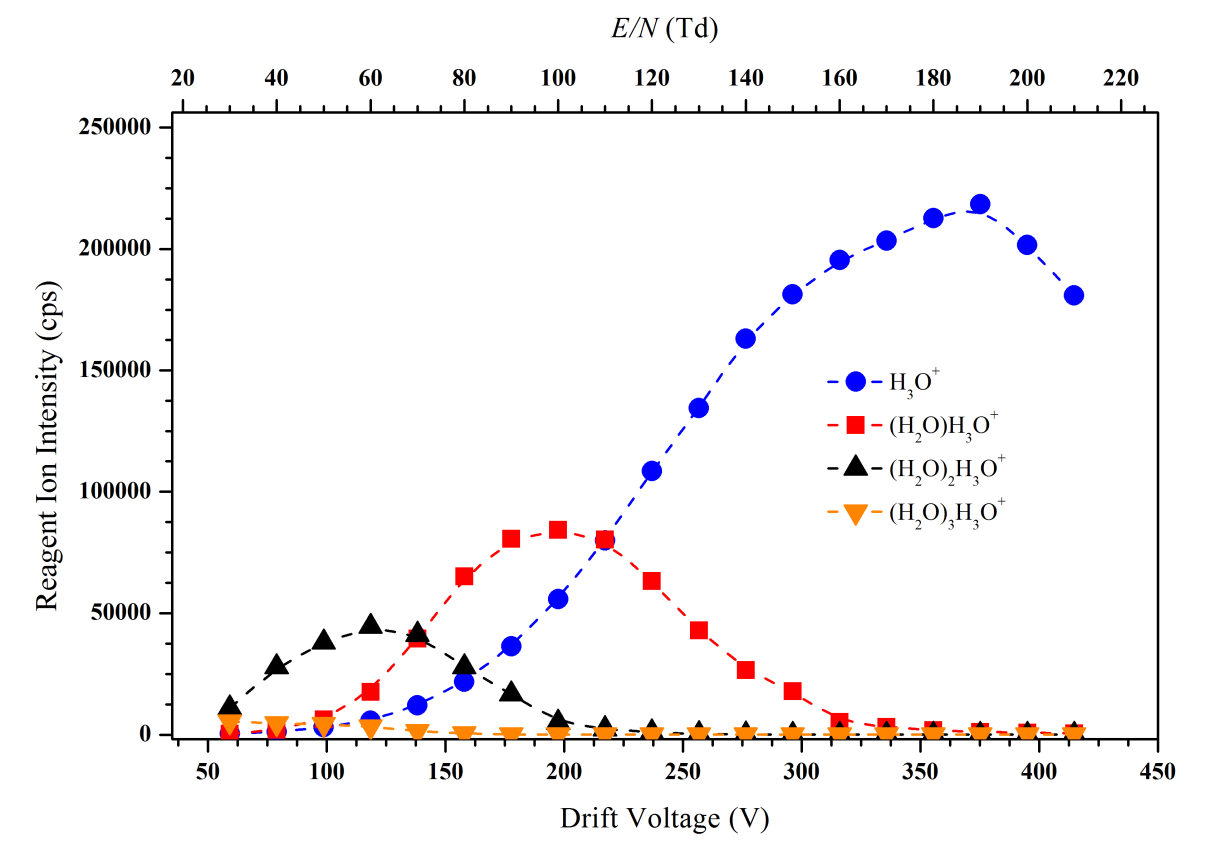
\includegraphics[width=0.60\linewidth]{pics/ISOF/ANAESTH_011.png}
}

\sidesubfloat[]{
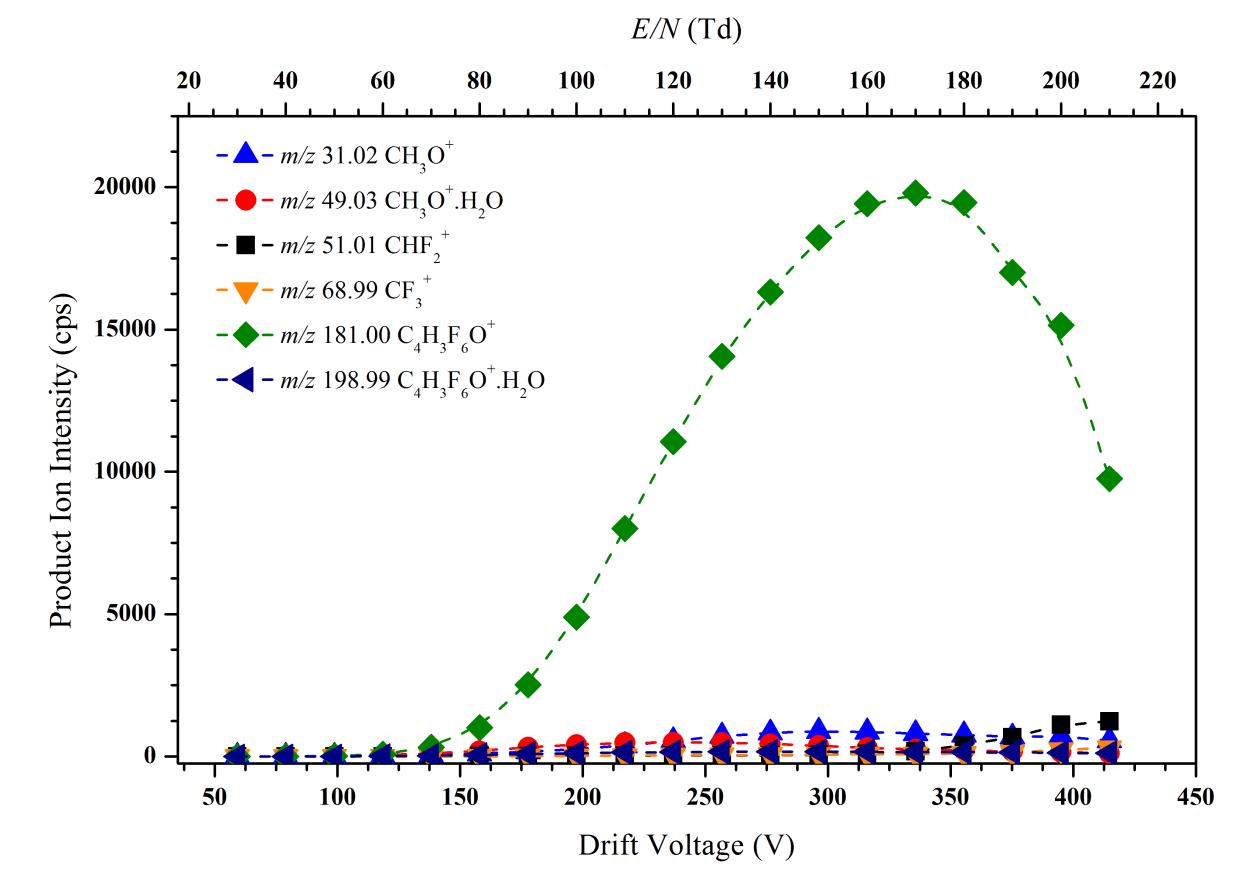
\includegraphics[width=0.60\linewidth]{pics/ISOF/ANAESTH_015.png}
}

\sidesubfloat[]{
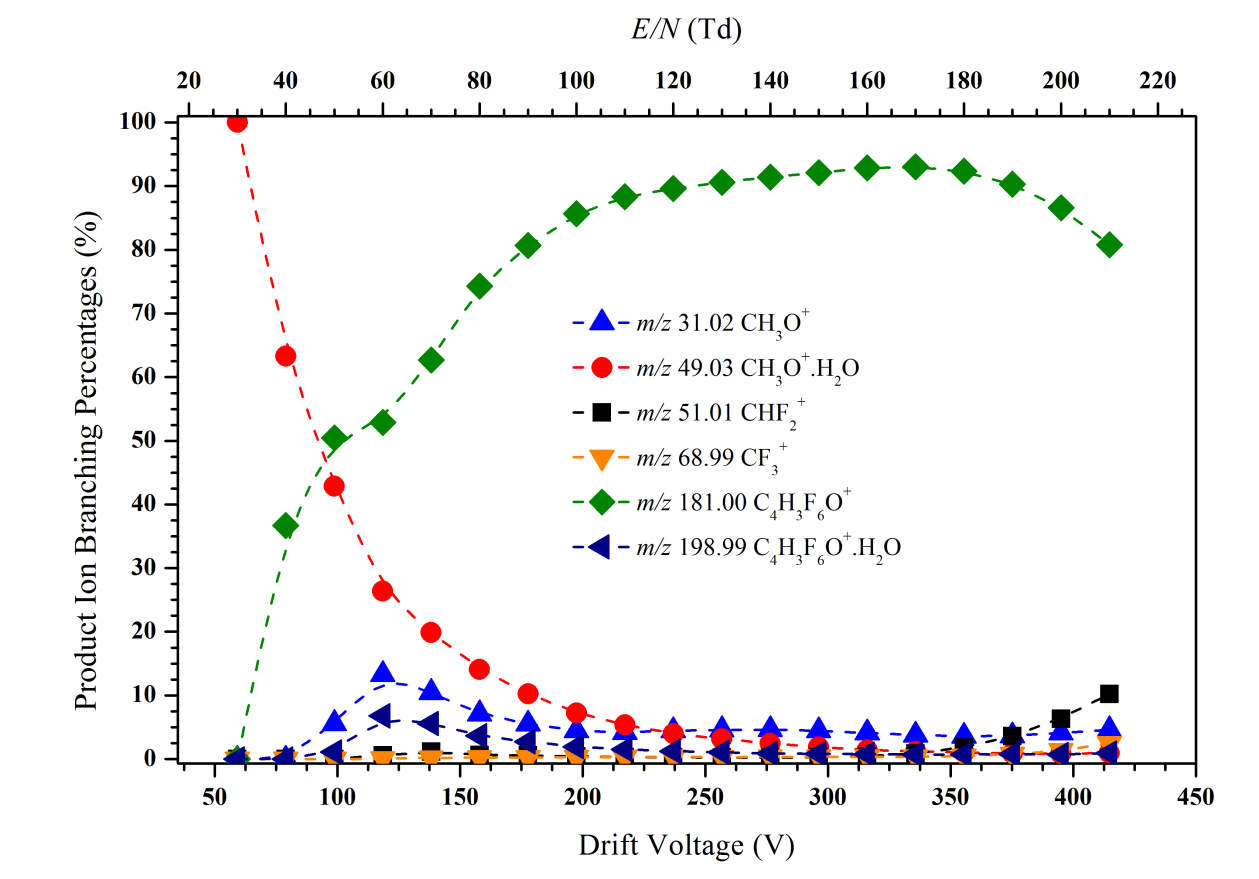
\includegraphics[width=0.60\linewidth]{pics/ISOF/ANAESTH_013.png}
}

\caption{(a) Reagent ions intensity plot and product ions  (b) intensity and (c) distribution plots from the reaction of sevoflurane and (H$_2$O)$_n$H$_3$O$^+$ in humid conditions.}
\label{fig:sevo_h3o_h}
\end{figure}





%\section{Introduction}
%\section{Methodology}
%\subsection{PTR-MS vs SIFT-MS vs SIFDT-MS}





%\subsubsection{Rate constants}
%%%The home-built \acrshort{sifdtms} instrument at the Heyrovsky Institute of Physical Chemistry of the Academy of Sciences in Prague (Czech Republic) has been described in detail elsewhere \cite{doi:10.1021/acs.analchem.5b02994}.

%The calculation of the rate constant comes from Su \cite{su1994parametrization}.

%The data for $\alpha$ and $\mu_D$ can be found in \cite{lide2012crc}.



%\begin{figure}%[h]
%\centering
%\sidesubfloat[]{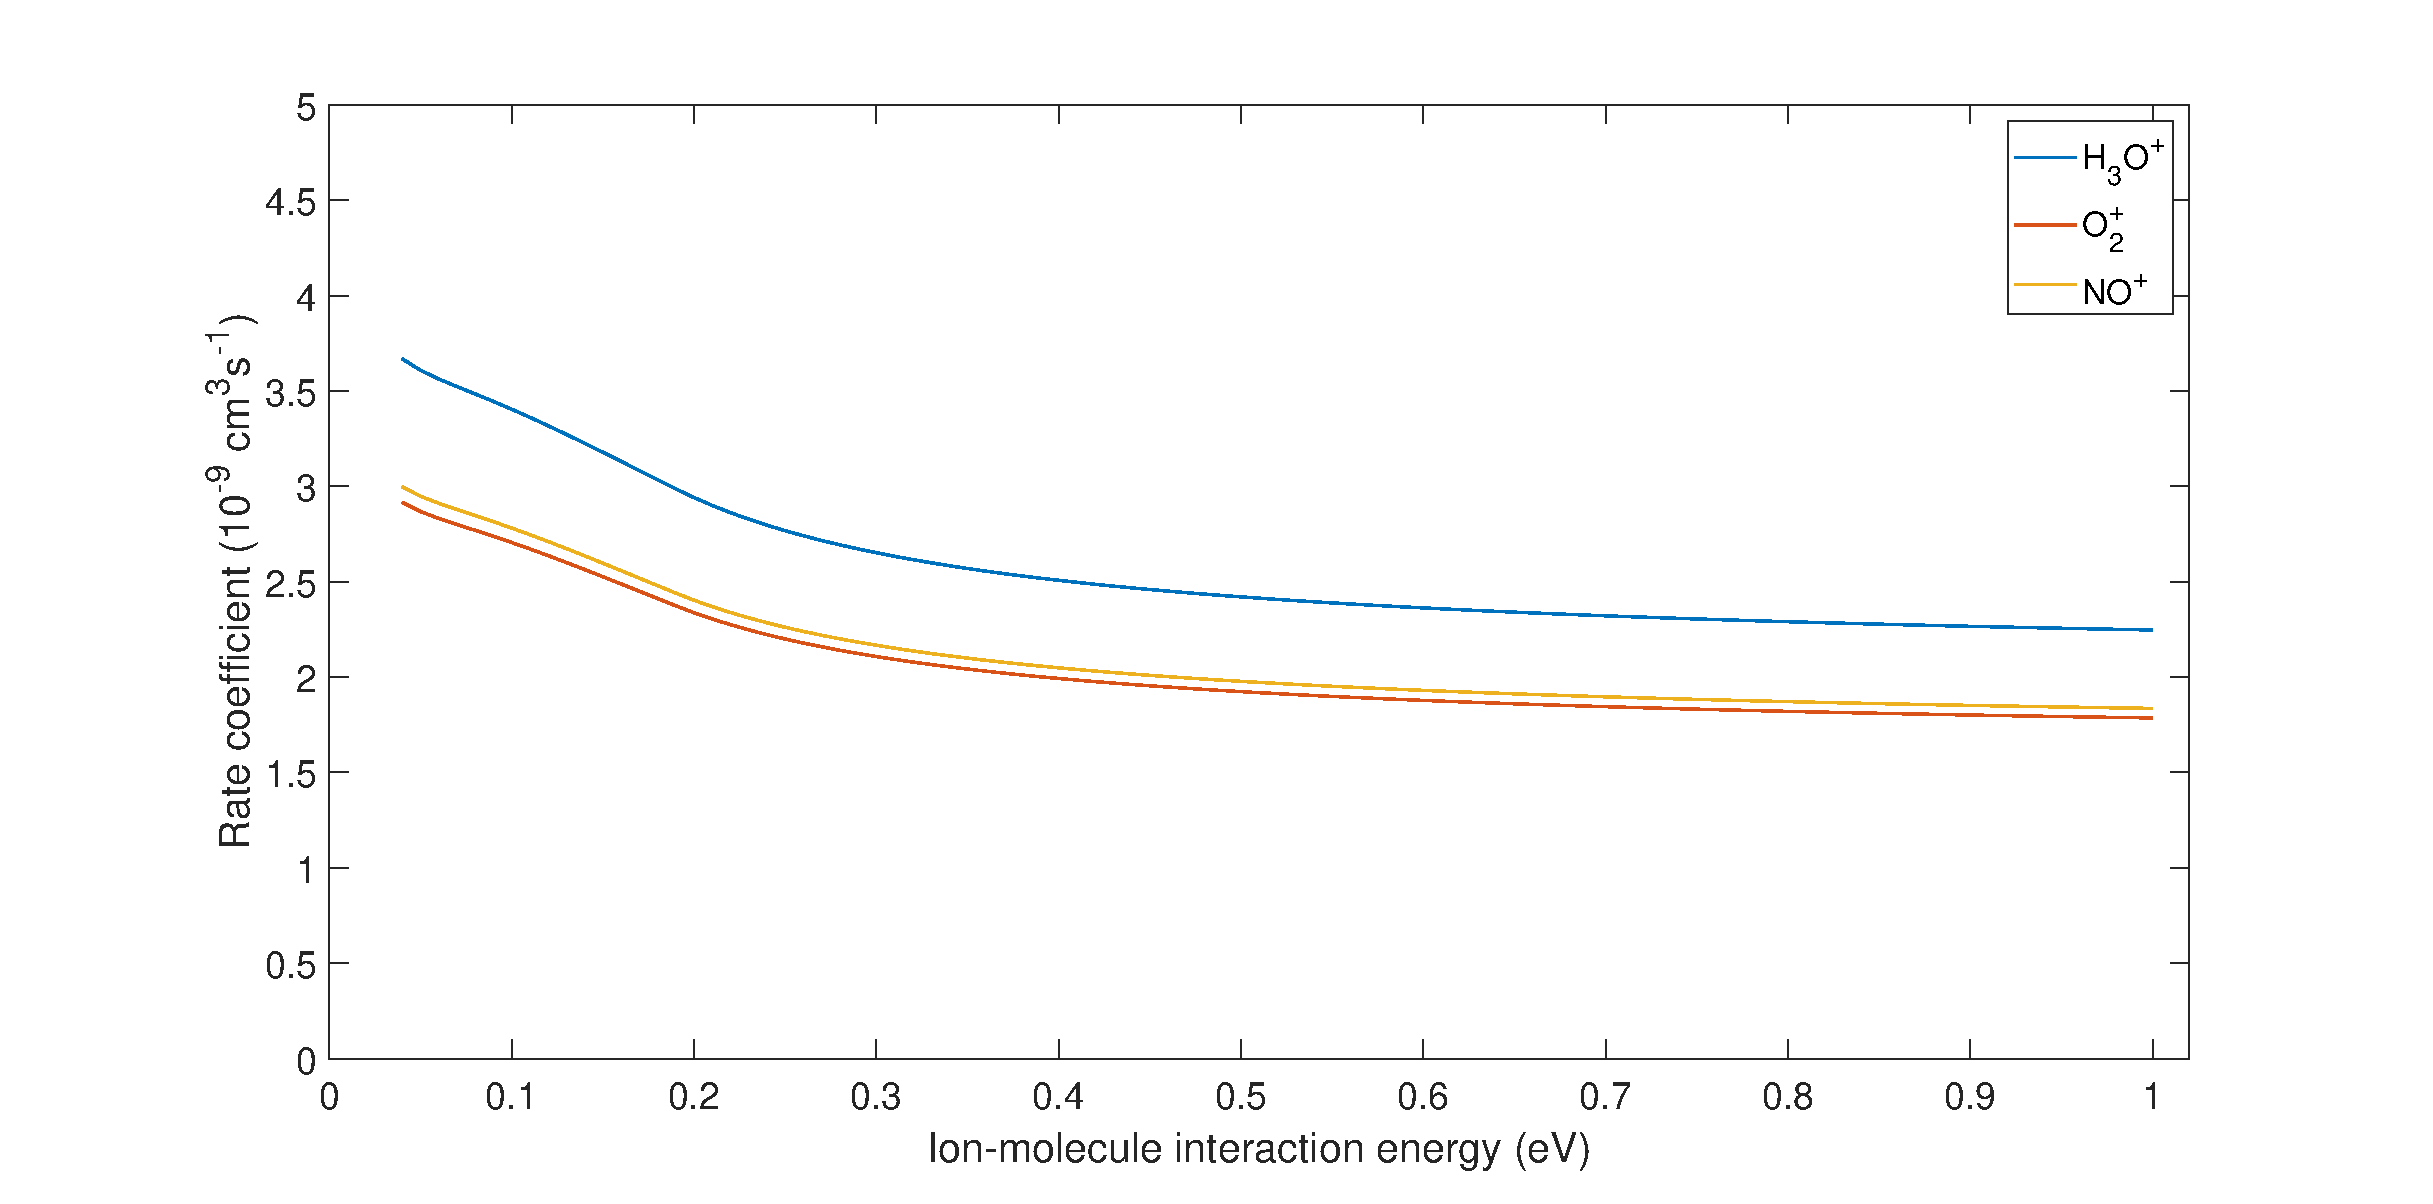
\includegraphics[width=0.9\linewidth]{pics/rate_constants_isoflurane.eps}}

%\sidesubfloat[]{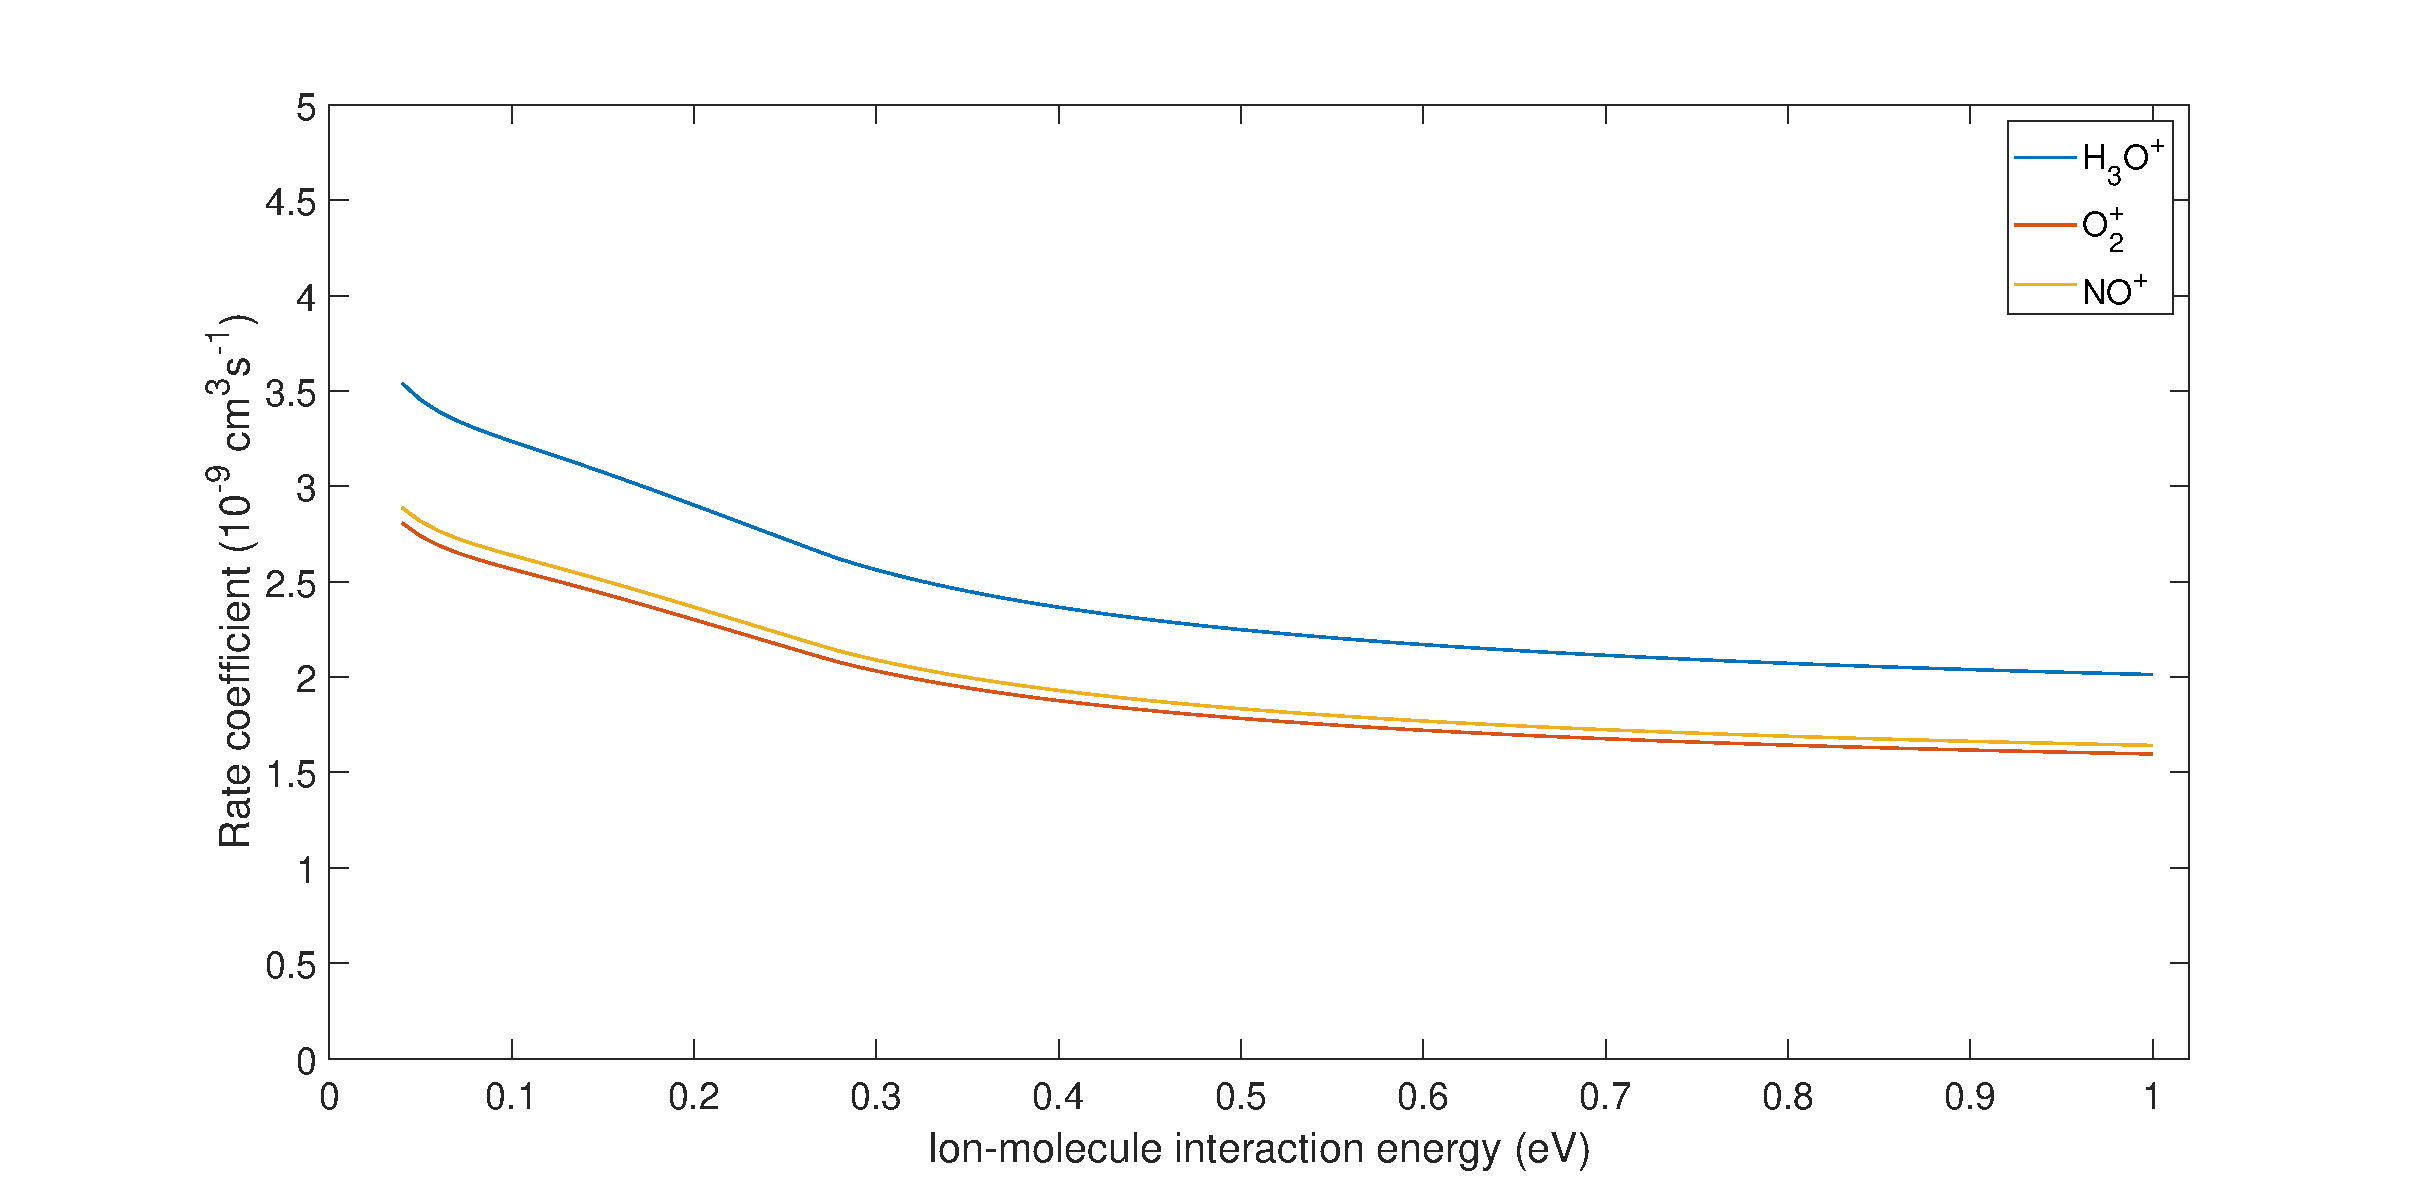
\includegraphics[width=0.9\linewidth]{pics/rate_constants_sevoflurane.eps}}
%\caption{Collisional rate coefficients of (a) isoflurane and (b) sevoflurane with different reagent ions as a function of the interaction energy as predicted by the Su model \cite{su1994parametrization}}
%    \label{fig:rate_iso_sevo}
%\end{figure}

%%%%%%%%%%%%%%%%%%%%%%%%%%%%%%%%%%%%%%%%%%%%%%%%%%%%%%%%%%%%%%%%%%%%%%%%%%%%%%%%%%%%%%%%%%%%%%%%%%%%

%\section{Concerns at the moment}
%There are some concerns regarding isoflurane:
%\begin{itemize}
%    \item It is very sensitive to humidity. In the past, people thought that the discrepancies in the PTRMS results from isoflurane measurements were due to the difference geometries of the instruments from different manufacturers, which raised doubts about the standardisation of PTRMS.
%    \item There is an ion reported at  \textit{m/z} 163 by \cite{smith2003analysis}. The energy required for its fragmentation it is too high, around 1.8 eV.
%    \item Furthermore, the ion assigned to  \textit{m/z} 147 does not have proper isotopic distribution (note that the scale is logarithmic and  \textit{m/z} 149 is not 1/3 of \textit{m/z}  147)
%\end{itemize}

%%%%%%%%%%%%%%%%%%%%%%%%%%%%%%%%%%%%%%%%%%%%%%%%%%%%%%%%%%%%%%%%%%%%%%%%%%%%%%%%%%%%%%%%%%%%%%%%%%%%





